\documentclass{article}
\usepackage{graphicx} % Required for inserting images
\usepackage[vietnamese]{babel}
\usepackage{vmargin}
\setmarginsrb{1.5 in}{2 cm}{1 in}{2 cm}{1 cm}{1 cm}{1 cm}{1 cm}
\usepackage{amsthm, amsmath, amssymb,amsfonts}
\usepackage{indentfirst}
\usepackage[colorlinks=true, linkcolor=black, urlcolor=blue, pdfborder={0 0 0}]{hyperref}
\usepackage{titling}
\usepackage{listings}
\usepackage{tocloft}
\usepackage{caption}
\usepackage{colortbl}
\usepackage[utf8]{inputenc}
\usepackage[final]{pdfpages}
%\usepackage{parskip}
\usepackage{fancyhdr}


\title{Channel Estimation}
\author{
  Phạm Võ Hiệp \\
  Mã Chí Nhân \\
  Bùi Thị Huyền Như\\
}
\date{\today}

\makeatletter
\let\thetitle\@title
\let\theauthor\@author
\let\thedate\@date
\makeatother

\pagestyle{fancy}
\fancyhf{}
\fancyhead[L]{\thetitle}
\fancyfoot[C]{\thepage}

\begin{document}

\begin{titlepage}
    \centering
    
\includegraphics[scale=0.35]{photo/logo.png}\\[1.0 cm]
    \textsc{\LARGE Trường Đại học Bách Khoa\\ Đại học Quốc gia TP.HCM}\\[1.5 cm]
    
    \textsc{\Large Bộ môn viễn thông}\\[0.5 cm]
    \textsc{\large Môn học: Kĩ thuật hệ thống viễn thông}\\[0.5 cm]
    \rule{\linewidth}{0.2 mm} \\[0.4 cm]
    {\huge \bfseries \thetitle}\\
    \rule{\linewidth}{0.2 mm} \\[1.5 cm]

    \begin{minipage}{0.4\textwidth}
        \begin{flushleft} \large
            \theauthor \\
            \vspace{0.3 cm}
            {\small Nhóm trưởng: Mã Chí Nhân\\}
            \textit{\small Gmail: nhan.ma1309@gmail.com}\\
            {\small Tel: 0948.108.474}
        \end{flushleft}
    \end{minipage}~
    \begin{minipage}{0.4\textwidth}
        \begin{flushright} \large
            \emph{2211051\\2212359\\2212464} \\
            \vspace{1 cm}
            {\small GVHD: Đặng Ngọc Hạnh}
        \end{flushright}    
    \end{minipage}\\[2 cm]
    
    {\large \thedate}\\[2 cm]

    \vfill
\end{titlepage}

\begin{center}
       Các chữ viết tắt và cách dịch được sử dụng\\
       \begin{tabular}{c|c|c}
        \hline
     Tên tiếng anh&Tên tiếng việt&Chữ viết tắt  \\
     \hline
     Single Input Single Output & Ngõ vào đơn ngõ ra đơn & SISO\\
     Multiple Input Multip;e Output& Đa ngõ vào đa ngõ ra& MIMO\\
     Multiple Input Single Output& Đa ngõ vào một ngõ ra &MISO\\
     Single Input Multiple Output& Đơn ngõ vào đa ngõ ra&SIMO\\
     Maximum Likelihood Estimation&Phương pháp ước lượng hợp lý cực đại&MLE\\
     Intelligent Reflecting Surfaces&Bề mặt phản xạ thông minh&IRS\\
     Channel Impulse Respond&Phản hồi xung kênh&CIR\\
     Least square&Bình phương tối thiểu&LS\\
     Compressed Sensing&Cảm biến nén&CS\\
     Discrete Fourier Transform&Biến đổi Fourier rời rạc&DFT\\
     Signal to Noise Ratio&Tỉ số tín hiệu trên nhiễu&SNR\\
     Linear Time-Invariant&Tuyến tính bất biến&LTI\\
     Imaginary part&Phẩn ảo của số phức&\mathcal{j}\\
     Frequency Division Multiplexing&Ghép kênh theo tần số &FDM\\
     Orthogonal Frequency Division Multiplexing&Ghép kênh theo tần số trực giao&OFDM\\
     Base Station& Trạm gốc&BS\\
     Line of Sight&Trong tầm ngắm&LoS\\
     Non-Light of Sight&Không trong tầm ngắm&NLoS\\
     Pilot signal&Tín hiệu hoa tiêu&\\
     Uncorrelated&Không tương quan&\\
     Covarriance&Hiệp phương sai&\\
     Hermitian transpose&Chuyển vị liên hợp phức&\\
     Ray Tracing&Phương pháp dò tia&\\

  
\end{tabular}

\end{center}
\newpage
\tableofcontents
\listoffigures
\newpage

\section{Giới thiệu}
\subsection{Đặt vấn đề}
Trong hệ thống thông tin viễn thông, việc truyền tải tín hiệu từ nguồn đến đích phụ thuộc rất lớn vào kênh truyền – môi trường mà tín hiệu sẽ đi qua. Kênh truyền không chỉ là một thành phần vật lý mà còn bao gồm các yếu tố môi trường gây ảnh hưởng đến tín hiệu như nhiễu, suy hao, phản xạ, tán xạ và băng thông hạn chế. Do đó, để đảm bảo chất lượng truyền tải và tính ổn định của hệ thống, ước lượng và mô hình hóa kênh truyền là một yêu cầu cấp thiết.\\

Ước lượng kênh truyền giúp nhận biết và đo lường các yếu tố ảnh hưởng lên tín hiệu trong quá trình truyền tải, từ đó cung cấp thông tin quan trọng cho việc hiệu chỉnh và tối ưu hóa hệ thống. Các kỹ thuật ước lượng kênh truyền đóng vai trò quyết định trong việc xác định chính xác các tham số của kênh, giúp các bộ giải mã ở đầu thu tái tạo tín hiệu gần đúng với tín hiệu gốc nhất có thể. Bên cạnh đó, ước lượng kênh còn góp phần cải thiện hiệu suất truyền thông, giảm tỷ lệ lỗi và tối ưu hóa hiệu năng của các kỹ thuật truyền dữ liệu hiện đại như MIMO, OFDM, FDM và các công nghệ truyền thông không dây thế hệ mới.\\

Tuy nhiên, quá trình ước lượng kênh truyền gặp nhiều thách thức lớn do sự thay đổi nhanh chóng và đa dạng của môi trường truyền dẫn, đặc biệt trong các hệ thống di động và không dây. Việc phát triển các kỹ thuật ước lượng hiệu quả và phù hợp với các điều kiện kênh khác nhau là vấn đề cấp thiết đặt ra cho ngành thông tin viễn thông. Báo cáo này sẽ trình bày về một vài phương pháp ước lượng kênh truyền phổ biến, phân tích các đặc điểm, ưu nhược điểm và ứng dụng của từng phương pháp, và thực hiện mô phỏng trên MATLAB.

\section{Một vài kỹ thuật ước lượng kênh truyền}
\subsection{Ước lượng hợp lý cực đại}
Phương pháp Maximum Likelihood (ML) nhằm tìm ước lượng đáp ứng tần số của kênh truyền sao cho xác suất xảy ra giá trị kênh truyền như ước lượng là lớn nhất, với điều kiện là các tham số bên phát và bên thu của kênh được cho trước.\\

Ta có một hệ thống MIMO với \( N_t \) anten phát và \( N_r \) anten thu. Tín hiệu thu được \( \mathbf{y} \) có thể mô hình hóa theo phương trình:

\[
\mathbf{y} = \mathbf{H} \mathbf{x} + \mathbf{n}
\]

Trong đó:
\begin{itemize}
  \item \( \mathbf{y} \) là vector tín hiệu thu,
  \item \( \mathbf{H} \) là ma trận kênh (kích thước \( N_r \times N_t \)),
  \item \( \mathbf{x} \) là vector tín hiệu phát,
  \item \( \mathbf{n} \) là vector nhiễu, giả sử theo phân phối Gaussian.
\end{itemize}

Mục tiêu của ước lượng kênh bằng Maximum Likelihood (ML) là tìm ma trận kênh \( \mathbf{H} \) sao cho xác suất mà \( \mathbf{H} \) xảy ra trong thực tế là lớn nhất. Phương trình ML sẽ tối ưu hóa hàm khả năng của mô hình này, từ đó ước lượng được \( \mathbf{\hat{H}} \).\\

Hàm hợp lý cực đại (Maximum Likelihood Function) là:

\[
\hat{h}_{\text{ML}} = \arg \max_h L(h; \mathbf{y})
\]

Trong đó:
\begin{itemize}
  \item \( L(h; \mathbf{y}) \) là hàm khả năng (likelihood function) của tham số kênh \( h \) 
  \item \( \hat{h}_{\text{ML}} \) là ước lượng tham số kênh tối ưu.
\end{itemize}

Hàm khả năng \( L(h; \mathbf{y}) \) được xác định bằng cách tính xác suất của dữ liệu quan sát \( \mathbf{y} \) trong một mô hình xác suất của kênh, dựa trên các tham số kênh \( h \).
\begin{figure}[h!]
    \centering
   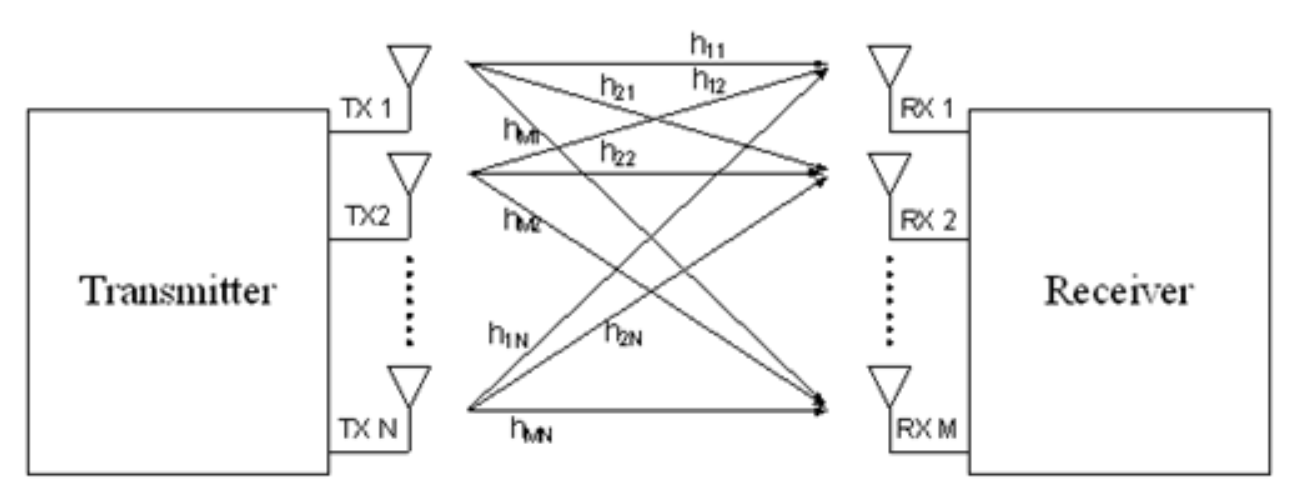
\includegraphics[width=14cm]{photo/2.1.png}
    \caption{Mô hình kênh truyền đa ngõ vào đa ngõ ra}
    \label{Hình 1}
\end{figure}

\subsubsection{Ưu điểm và nhược điểm}
\subparagraph{Ưu điểm}

\begin{itemize}
    \item {Độ tin cậy cao:}\\ Phương pháp ML cung cấp ước lượng tối ưu trong nghĩa thống kê, vì nó tối đa hóa xác suất quan sát dữ liệu thực tế dựa trên mô hình kênh và nhiễu.
    \item {Ứng dụng Rộng:}\\ Có thể áp dụng cho nhiều loại mô hình kênh khác nhau, từ kênh đơn giản như SISO, SIMO đến các kênh phức tạp như MIMO (Multiple Input, Multiple Output) với điều kiện nhiễu Gaussian.
    \item Dễ dàng tính toán, dễ dàng thực hiện:\\ Vì các phương trình trong phương pháp này đều là tuyến tính nên các phép toán chỉ xoay quanh nhân ma trận và vector.
\end{itemize}

\subparagraph{Nhược điểm}

\begin{itemize}

    \item {Tốn công suất đối với những kênh quá phức tạp và băng thông lớn:}\\ Đối với hệ thống MIMO lớn, mỗi bên phát sẽ cần một tín hiệu hoa tiêu tại một tần số, dẫn đến số lượng tín hiệu hoa tiêu cần phát đi rất nhiều gây hao phí công suất. Khi muốn ước lượng một kênh truyền có băng thông lớn, mỗi bên phát sẽ phải phát đi nhiều tần số khác nhau và các giá trị tần số bị khuyết sẽ được nội suy từ những tần số có thể ước lượng, dẫn đến sai số tại các tần số nội suy
    \item {Yêu cầu dữ liệu đủ lớn:}\\ Do đặc thù là một phương pháp ước lượng bằng thống kê. Nên ML yêu cầu dữ liệu mẫu quan sát đủ lớn và chính xác để có thể ước lượng được một tổng thể với độ tin cậy cao.
    \item Chỉ hiệu quả với kênh truyền LoS:\\ Trong kênh truyền LoS, tín hiệu hoa tiêu từ bên phát có thể đi đến bên thu mà vẫn còn duy trì một công suất đủ lớn. Khi kênh truyền là NLoS, SNR lúc này sẽ rất nhỏ và tín hiệu nhận được bị trộn với nhiễu và không còn có thể khôi phục tín hiệu gốc
    \item Không tương thích với kênh truyền động:\\ Trong kênh truyền động, khi bên nhận hoặc bên phát thay đổi vị trí, kênh truyền đến các bên khác cũng sẽ bị ảnh hưởng. Vì vậy, để ước lượng được kênh truyền động theo ML, ta phải liên tục phát tín hiệu hoa tiêu và tính toán kênh truyền, gây tổn hao công suất phát và năng lực tính toán của vi xử lý
\end{itemize}
\begin{center}
    \begin{tabular}{c|c}
    
     \textbf{Ưu điểm}&\textbf{Nhược điểm}\\ 
     \hline
     Độ tin cậy cao&Tốn công suất với kênh băng thông rộng\\
     Ứng dụng rộng & Yêu cầu dữ liệu đủ lớn\\
     Dễ dàng tín toán&Chỉ hiệu quả với kênh LoS\\
     &Không tương thích với kênh truyền động\\
\end{tabular}
\end{center}

\subsubsection{Ứng Dụng}
\begin{itemize}

\item Trong các hệ thống MIMO, nơi có nhiều anten cả ở phía phát và phía thu. Tồn lại nhiễu kênh truyền khác nhau tác động qua lại giữa bên phát và bên thu, và ML giúp ước lượng các hệ số kênh này một cách tối ưu.
\item Trong các hệ thống tĩnh như giữ các trạm phát sóng, với các hệ thống mà môi trường giữa bên phát và bên thu không bị thay đổi quá nhiều theo thời gian, việc ước lượng ML sẽ cho ra giá trị kênh truyền đáng tin cậy trong thời gian dài
\item Trong các hệ thống kênh ghép theo tần số, ML có thể ước lượng được đáp ứng tần số ở khoảng băng thông lớn, điều này rất cần thiết trong các kỹ thuật ghép tần số như FDM, OFDm,..

\end{itemize}

\subsection{Ước lượng dựa vào cảm biến nén - Compressed Sensing}

Trong các hệ thống MIMO khổng lồ, số lượng liên kết và kênh không dây rất lớn, dẫn đến sự gia tăng tín hiệu hoa tiêu, tăng chi phí thu thập dữ liệu và ước lượng. Tuy nhiên, kênh không dây về cơ bản là thưa, trong đó chỉ có một số ít hệ số kênh là khác không. Do vậy, để giảm chi phí tín hiệu điều khiển, một lựa chọn tiềm năng là áp dụng kỹ thuật nén dữ liệu, ước lượng kênh thưa có thể được sử dụng để ước lượng phản hồi xung kênh dựa trên các ký tự điều khiển nhận và truyền. So với các phương pháp bình phương tối thiểu và sai số trung bình tối thiểu (MMSE), ước lượng kênh thưa có khả năng cải thiện hiệu suất ước lượng kênh và giảm chi phí tín hiệu điều khiển.\\

\begin{figure}[h!]
    \centering
    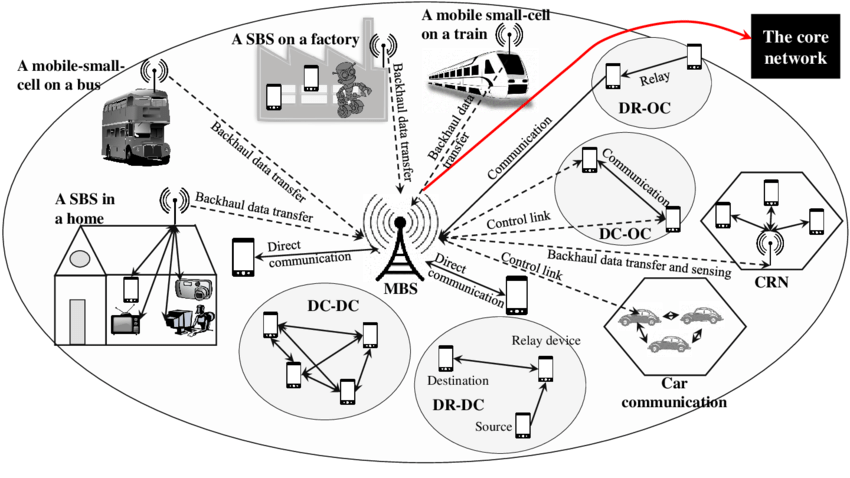
\includegraphics[width=10cm]{photo/2.2.png}
    \caption{Mô hình MIMO quy mô lớn}
    \label{Hình 2}
\end{figure}

\newpage


\subsubsection{Mô hình Cảm Biến Nén}

 Trong Cảm Biến Nén, thay vì thu thập tín hiệu một cách đầy đủ toàn bộ tín hiệu hoa tiêu như ML, chúng ta chỉ thu thập một số lượng mẫu rất ít (ít hơn nhiều so với số lượng điểm cần thiết trong lý thuyết Nyquist-Shannon), nhưng thông qua một phép đo tuyến tính. Sau đó, bằng cách sử dụng các thuật toán phục hồi tín hiệu, ta có thể tái tạo lại tín hiệu gần đúng với độ chính xác cao.\\

 Các tín hiệu có thể được xem là thưa trong một cơ sở biến đổi (như DFT, wavelet, hay biến đổi cosine), và việc tái tạo tín hiệu chỉ yêu cầu ít mẫu từ các phép đo này, miễn là các điều kiện về độ thưa của tín hiệu và các phép đo được đáp ứng.\\

\subsubsection{Các Công Thức và Biểu Thức Toán Học Chính}

 Mô Hình Cảm Biến Nén
Giả sử có một tín hiệu \( \mathbf{s} \in \mathbb{R}^N \) và tín hiệu này có thể được biểu diễn dưới một cơ sở thưa nào đó (ví dụ: qua phép biến đổi wavelet, DCT, DFT). Tín hiệu này có thể viết lại dưới dạng:

\[
\mathbf{x} = \mathbf{\Phi} \mathbf{s}
\]

Trong đó:
\begin{itemize}
  \item \( \mathbf{s} \in \mathbb{R}^N \) là tín hiệu ban đầu.
  \item \( \mathbf{\Phi} \in \mathbb{R}^{N \times N} \) là ma trận cơ sở mà tín hiệu được biểu diễn trong đó.
  \item \(  \mathbf{x} \in \mathbb{R}^N \) là một vector thưa, với nhiều phần tử bằng 0.
\end{itemize}

Trong trường hợp thực tế, ta chỉ thu thập một phần của tín hiệu \( \mathbf{x} \), gọi là các phép đo.\\

 Lấy Mẫu Tín Hiệu:
Cảm biến nén sẽ thu thập các phép đo từ tín hiệu \( \mathbf{x} \), thông qua một ma trận \( \mathbf{A} \in \mathbb{R}^{M \times N} \), với \( M < N \), tức là số lượng phép đo \( M \) ít hơn số chiều của tín hiệu \( N \). Các phép đo này được tính bằng:

\[
\mathbf{y} = \mathbf{A} \mathbf{x} + \boldsymbol{\epsilon}
\]

Trong đó:
\begin{itemize}
  \item \( \mathbf{y} \in \mathbb{R}^M \) là vector các phép đo.
  \item \( \mathbf{A} \in \mathbb{R}^{M \times N} \) là ma trận phép đo.
  \item \( \boldsymbol{\epsilon} \in \mathbb{R}^M \) là sai số nhiễu (nếu có).
\end{itemize}

Vì \( M \) nhỏ hơn \( N \), đây là một hệ phương trình không đầy đủ. Tuy nhiên, nếu tín hiệu \( \mathbf{x} \) là thưa, tức là nó có thể được biểu diễn gần đúng với một số ít các thành phần không bằng 0 trong cơ sở \( \mathbf{\Phi} \), ta có thể phục hồi lại tín hiệu \( \mathbf{x} \) từ các phép đo \( \mathbf{y} \).\\

 Phục Hồi Tín Hiệu Thưa
Với giả định rằng tín hiệu \( \mathbf{x} \) là thưa (chỉ có một số lượng nhỏ phần tử không bằng 0 trong cơ sở \( \mathbf{\Phi} \)), bài toán phục hồi tín hiệu có thể được mô tả như một bài toán tối ưu. Mục tiêu là tìm tín hiệu \( \mathbf{x} \) sao cho nó gần với các phép đo \( \mathbf{y} \), đồng thời đảm bảo rằng \( \mathbf{x} \) là thưa. Bên cạnh đó, kết hợp phương pháp L1 Minimization\\

Bài toán khôi phục có thể viết dưới dạng:

\[
\hat{\mathbf{x}} = \arg \min_{\mathbf{x}} \left\| \mathbf{A} \mathbf{x} - \mathbf{y} \right\|_2^2 + \lambda \left\| \mathbf{x} \right\|_1
\]

Trong đó:
\begin{itemize}
 \item \( \left\| \mathbf{A} \mathbf{x} - \mathbf{y} \right\|_2^2 \) là sai số giữa phép đo thực tế và dự đoán.
  \item \( \left\| \mathbf{x} \right\|_1 \) là tổng giá trị tuyệt đối của các phần tử trong \( \mathbf{x} \), là một cách để đo độ thưa của tín hiệu.
  \item \( \lambda \) là một tham số điều chỉnh độ mạnh của ràng buộc L1.
\end{itemize}

\subsubsection{Ưu và nhược điểm của Compressed Sensing}
\subparagraph{Ưu điểm}
\begin{itemize}
\item Giảm tải tin hiệu hoa tiêu và năng lượng:\\
Một trong những lợi ích chính của CS là cho phép ước lượng kênh thưa một cách chính xác với số lượng tín hiệu hoa tiêu ít hơn so với các phương pháp ước lượng kênh truyền thống, CS giúp tiết kiệm năng lượng. 

\item Tính linh hoạt và khả năng mở rộng:\\
Các kỹ thuật CS có thể mở rộng để xử lý các bài toán ước lượng kênh có kích thước lớn. Ví dụ, trong các hệ thống MIMO bằng cách lắp đặt thêm các cảm biến, CS có thể ước lượng kênh hiệu quả với ít tài nguyên đầu tư, làm cho nó trở thành sự lựa chọn tốt cho các hệ thống quy mô trải rộng.

\item Giảm số lượng mẫu cần xử lý:\\
Vì ít tín hiệu hoa tiêu hơn được yêu cầu, nên số lượng mẫu cần lưu trữ và xử lý sẽ ít hơn đáng kể so mới lương pháp ML.
\end{itemize}

\subparagraph{Nhược điểm}
\begin{itemize}
\item Độ phức tạp tính toán cao:\\
Việc giải các bài toán tối ưu như L1 minimization (chẳng hạn như thông qua Basis Pursuit hoặc các thuật toán khác) thường yêu cầu tài nguyên tính toán đáng kể, điều này có thể không thực tế cho các hệ thống thời gian thực với tài nguyên hạn chế, đặc biệt là trên các thiết bị di động hoặc thiết bị đầu cuối.

\item Mất thông tin:\\
Quá trình nén tín hiệu có thể dẫn đến mất một số thông tin về kênh. Điều này có thể ảnh hưởng đến độ chính xác của ước lượng nếu số lượng phép đo quá ít hoặc nếu các giả định về độ thưa không được thực hiện đúng. Trong một số trường hợp cực đoan, việc sử dụng quá ít phép đo có thể dẫn đến một ước lượng kênh sai lệch.

\item Thách thức trong triển khai thực tế:\\
Mặc dù CS lý thuyết cho kết quả xuất sắc trong các tình huống tín hiệu thưa, việc triển khai nó trong các hệ thống thực tế có thể gặp nhiều khó khăn. Bao gồm các vấn đề như độ chính xác của cảm biến, ảnh hưởng nhiễu không đồng bộ, bảo trì các cảm biến.

\end{itemize}

\begin{table}[h!]
\centering
\begin{tabular}{c|c}

\rowcolor{white} \textbf{Ưu điểm} & \textbf{Nhược điểm} \\ \hline
Giảm tải tín hiệu hoa tiêu và năng lượng & Độ phức tạp tính toán cao \\ 
Giảm số lượng mẫu xử lý và lưu trữ& Vấn đề trong triển khai thực tế \\  
Tính linh hoạt và khả năng mở rộng & Mất thông tin trong quá trình nén \\ 

\end{tabular}

\end{table}\\
\subsubsection{Một số ứng dụng}\\

Compressed Sensing hỗ trợ tối ưu hóa hiệu suất trong hệ thống truyền thông. Nén và truyền tín hiệu giúp giảm tải lượng dữ liệu cần truyền hoặc cần nhận để có thể khôi phục tín hiệu gốc.
\begin{itemize}
    \item Truyền dẫn tín hiệu thưa thớt CS cho phép giảm số lượng mẫu cần thu thập mà vẫn duy trì khả năng tái tạo đầy đủ tín hiệu, tiết kiệm năng lượng truyền tải.
    \item Trong hệ thống MIMO, CS được sử dụng để giảm số lượng thông tin cần thiết trong việc xác định ma trận kênh, từ đó giảm thời gian xử lý và khối lượng xử lý cần dữ liệu.
    \item Trong OFDM ứng dụng để giải mã tín hiệu, vì đặc tính thưa trong miền thời gian của kỹ thuật OFDM, CS có thể giúp tối ưu giải mã trong phương pháp này
    \item Ứng dụng trong truyền thông dữ liệu như hình ảnh và video.
\end{itemize}
\subsection{Phương pháp bộ lọc Kalman - Kalman Filtering}

Trong thực tế, các bên truyền nhận không phải lúc nào cũng cố định mà sẽ có các giai đoạn bên truyền và bên nhận sẽ thay đổi theo thời gian chẳng hạn như truyền thông giữa trạm phát và điện thoại của người dùng, giữa vệ tinh và các trạm phát trên trái đất,... Vì vậy, kênh truyền giữa chúng cũng sẽ liên tục thay đổi. Phương pháp bộ lọc Kalman giúp ước lượng ở đây là kênh truyền theo thời gian, dựa trên thông tin về các trạng thái và quan sát trước đó, cùng với mô hình động học của hệ thống.\\

\begin{figure}[h]
    \centering
   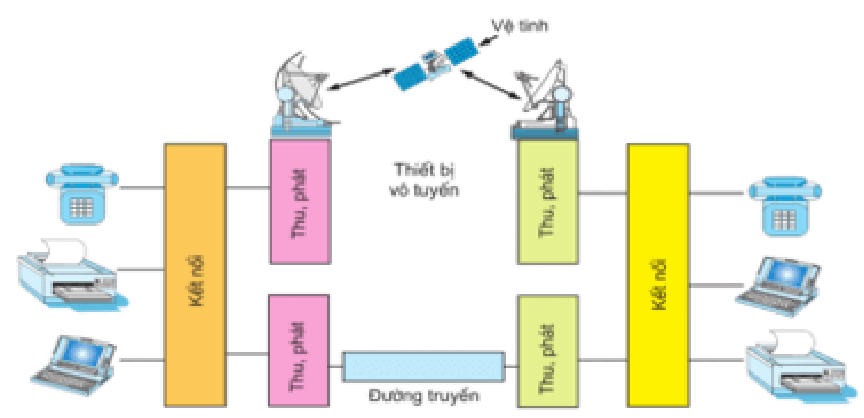
\includegraphics[width=12cm, height =6cm]{photo/2.3.1.png}
    \caption{Mô hình mạng lưới viễn thông}
    \label{Hình 3}
\end{figure}


\subsubsection{Mô hình toán học của phương pháp bộ lọc Kalman}
Bộ lọc Kalman thực hiện ước lượng trạng thái hiện tại của một hệ thống động dựa trên một mô hình quá trình (process model) và mô hình quan sát (observation model). Phương pháp này hoạt động thông qua hai bước chính:
Đầu tiên sẽ dự đoán (Prediction Step): Ước lượng trạng thái và sai số của nó tại thời điểm tiếp theo dựa trên trạng thái hiện tại và mô hình động học của hệ thống. Tiếp theo là cập nhật (Update Step): Điều chỉnh ước lượng trạng thái dựa trên quan sát thực tế mới nhất và ước lượng sai số, giúp cải thiện độ chính xác của dự đoán.\\

\begin{figure}[h!]
    \centering
    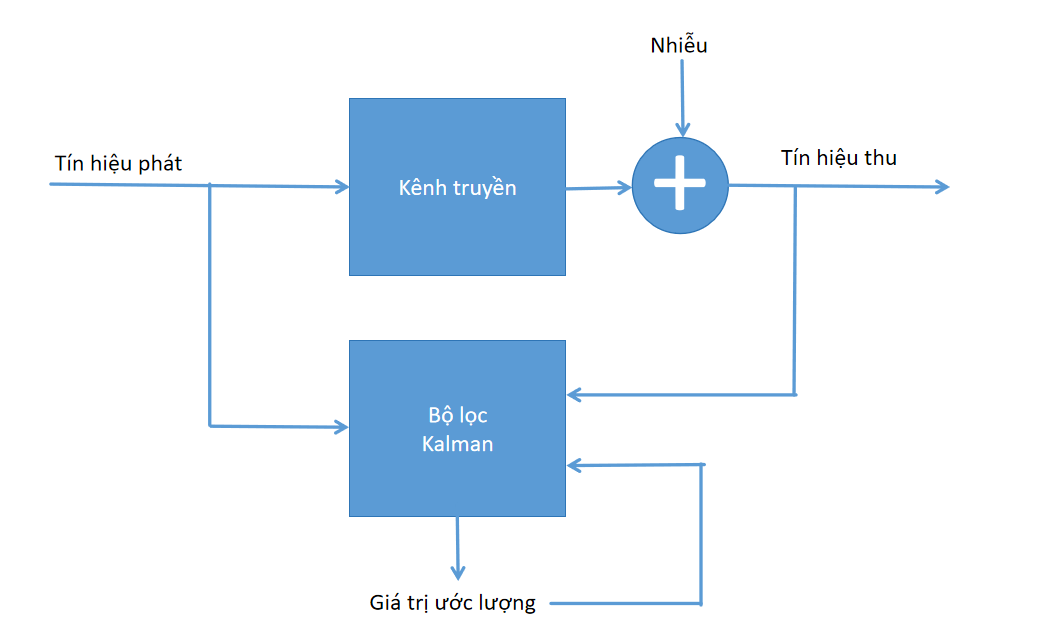
\includegraphics[width=13cm, height =8cm]{photo/2.3.2.png}
    \caption{Mô hình bộ lọc Kalman}
    \label{Hình 4}
\end{figure}
\newpage
Công thức mô tả sự biến đổi của trạng thái theo thời gian trong một hệ thống động có nhiễu. Đây là là một phần của mô hình trạng thái trong bộ lọc Kalman, giúp dự đoán trạng thái tiếp theo của hệ thống dựa trên trạng thái hiện tại, kích thích đầu vào và các yếu tố nhiễu.\\

    $$\dot{x}(t) = \frac{dx}{dt} = Ax(t) + Bu(t) + w(t)$$
    $$\text{Với }\begin{cases}
        \dot{x}(t) \text{Sự thay đổi của trạng thái hệ thống theo thời gian.}&\\
        x(t) \text{: vector trạng thái của hệ thống tại thời điểm }t&\\
        A \text{: Ma trận chuyển trạng thái, mô tả sự thay đổi của trạng thái qua thời gian}&\\
        u(t) \text{: vector điều khiển đầu vào tại thời điểm }t&\\
        B \text{: Ma trận tác động của đầu vào lên trạng thái hiện tại}&\\
        w(t) \text{ Nhiễu quá trình, được giả định là nhiễu trắng Gaussian}
    \end{cases}$$
    
Công thức mô tả mô hình quan sát thu được trong không gian trạng thái, thể hiện mối quan hệ giữa biến quan sát $y(t_i)$ dựa vào trạng thái hệ thống $x(t_i)$, kích thích đầu vào $u(t_i)$ và nhiễu $w(t_i)$ tại thời điểm $t_i$ cụ thể
$$y(t_i) = C.x(t_i) + D.u(t) + w(t_i)$$
$$\text{Với } \begin{cases}
    y(t_i) \text{: Vector quan sát tại thời điểm }t_i&\\
    x(t_i) \text{: Vector trạng thái của hệ thống tại thời điểm} t_i&\\
    C \text{: Ma trận quan sát, mô tả cách các trạng thái ảnh hưởng đến các quan sát}&\\
    u(t_i) \text{: vector điều khiển đầu vào tại thời điểm }t_i&\\
    D \text{: Ma trận đầu vào, cho biết ảnh hưởng của đầu vào lên quan sát}&\\
    w(t_i) \text{: Nhiễu quan sát tại thời điểm } t_i
\end{cases}$$

    
\subsubsection{Ưu điểm và nhược điểm của phương pháp bộ lọc Kalman }
\subparagraph{Ưu điểm}
\begin{itemize}
\item  Tối ưu hóa độ chính xác:\\
Bộ lọc Kalman được tối ưu hóa độ chính xác cho môi trường nhiễu trắng phân phối chuẩn, cho phép ước lượng trạng thái của hệ thống với độ chính xác cao, ngay cả trong các hệ thống có nhiễu.

\item Hiệu Quả Tính Toán:\\
Bộ lọc Kalman có cấu trúc lặp đơn giản và các phép tính tuyến tính, dễ dàng triển khai trong các ứng dụng thời gian thực. Tính chất này giúp bộ lọc trở thành lựa chọn lý tưởng cho các hệ thống cần ước lượng nhanh như điều khiển tự động và theo dõi đối tượng.

\item Khả năng theo dõi các hệ thống động:\\
Bộ lọc Kalman được thiết kế để cập nhật trạng thái liên tục theo thời gian, giúp nó thích ứng tốt với các hệ thống động hoặc môi trường thay đổi, chẳng hạn như theo dõi quỹ đạo chuyển động của các vật thể hoặc điều chỉnh các thông số hệ thống trong truyền thông không dây.
\end{itemize}
\subparagraph{Nhược điểm}
\begin{itemize}
\item Bị giới hạn trong môi trường phi truyến và nhiễu không phân phối chuẩn:\\
Bộ lọc Kalman được thiết kế cho các hệ thống tuyến tính và nhiễu phân phối chuẩn. Nếu hệ thống có tính phi tuyến hoặc nhiễu phi không phần phối chuẩn, hiệu suất của bộ lọc Kalman có thể giảm đáng kể. 

\item Nhạy cảm với điều kiện ban đầu:\\
Bộ lọc Kalman yêu cầu ước lượng trạng thái và hiệp phương sai lỗi ban đầu. Nếu các giá trị này được thu thập không chính xác hoặc vì một lý do nào đó mà điều kiện biên sai lệch lớn thì bộ lọc có thể mất nhiều thời gian để hội tụ về giá trị chính xác hoặc có thể dẫn đến sai lệch trong các ước lượng.
\item Tốn thơi gian xử lý:
Do phương pháp bộ lọc Kalman sử dụng kết quả là trạng thái hiện tại để dự đoán cho trạng thái kế tiếp. Do đó, để đảm bảo độ chính xác thì cần thời gian để các phương trình hội tự về nghiệm có sai số chấp nhận được.
\end{itemize}

\begin{center}
    \begin{tabular}{c|c}
         \textbf{Ưu điểm}&\textbf{Nhược điểm}  \\
         \hline
         Giảm thiểu tác động do nhiễu&Hạn chế ở môi trường phi tuyến\\
         Tính toán đơn giản đo & Nhạy cảm với điều kiện ban đầu\\
         Theo dõi được hệ thống động & Tốn thời gian để ước lượng hội tụ \\

    \end{tabular}
\end{center}
\subsection{Phương pháp dò tia - Ray Tracing}
\subsubsection{Phương pháp bề mặt phản xạ thông minh - Intelligent Reflecting Surfaces}
\paragraph{Mô hình của phương pháp IRS} Trong hệ thông viễn thông hiện đại, khoảng cách truyền thông tin càng ngày càng tăng lên để đảm bảo vùng phủ sóng. Tuy nhiên, sẽ có lúc các tín hiệu phát sẽ không thể trực tiếp đến được bên nhận vì nhiều lý do. Có thể là do giới hạn của hình dạng trái đất khiến cho tín hiệu giữa bên truyền và bên nhận không còn có thể di chuyển trực tiếp hoặc phải duy chuyển qua môi trường suy hao rất lớn như trong lòng trái đất. Cũng có thể tín hiệu nằm trong môi trường truyền dẫn nhiều vật cản dẫn đến phần lớn công suất bị phản xạ, tán xạ trước khi đến được điểm thu. Do đó, kỹ thuật sử dụng các bề mặt phản xạ thông minh được ứng dụng để truyền tín hiệu hiệu quả hơn và có thể tùy chỉnh kênh truyền cho mục đích sử dụng.\\

\begin{figure}[h!]
    \centering
    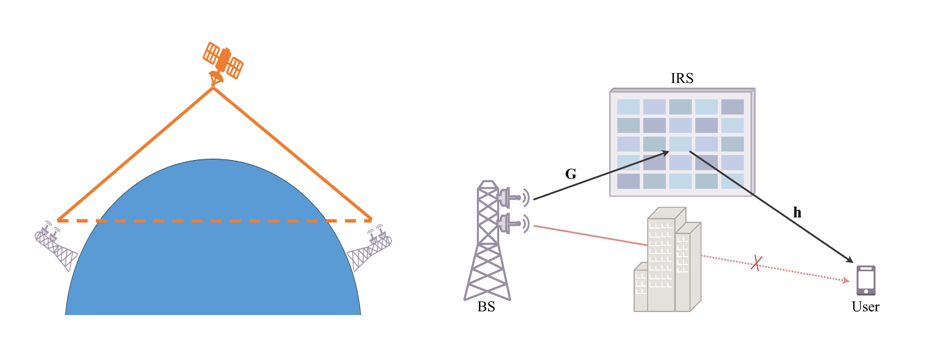
\includegraphics[width =14cm, height = 6cm]{photo/2.4.1.png}\\
   \caption{Truyền tín hiệu không trực tiếp}
    \label{Hình 5}
\end{figure}
\newpage
Cấu trúc của bề mặt phản xạ thông minh gồm: Bề mặt phản xạ chứa các phần tử phản xạ có thể điều hướng và bộ điều khiển trung tâm. Bề mặt phản xạ là một tấm phẳng, thường được gắn trên các bề mặt như tường hoặc trần, với các phần tử nhỏ gọi là "meta-elements" hoặc "meta-atoms". Các phần tử này có  thể điều chỉnh để thay đổi pha, cường độ, và hướng của tín hiệu phản xạ. Các phần tử này thường được chế tạo từ vật liệu có khả năng thay đổi điện từ (ví dụ: vật liệu kim loại, kính, tinh thể lỏng,...). Bộ điều khiển trung tâm: Một bộ điều khiển kết nối với các phần tử của IRS để điều chỉnh chúng theo thời gian thực dựa trên môi trường và mục tiêu cần truyền tín hiệu đến.\\
\begin{figure}[h!]
    \centering
    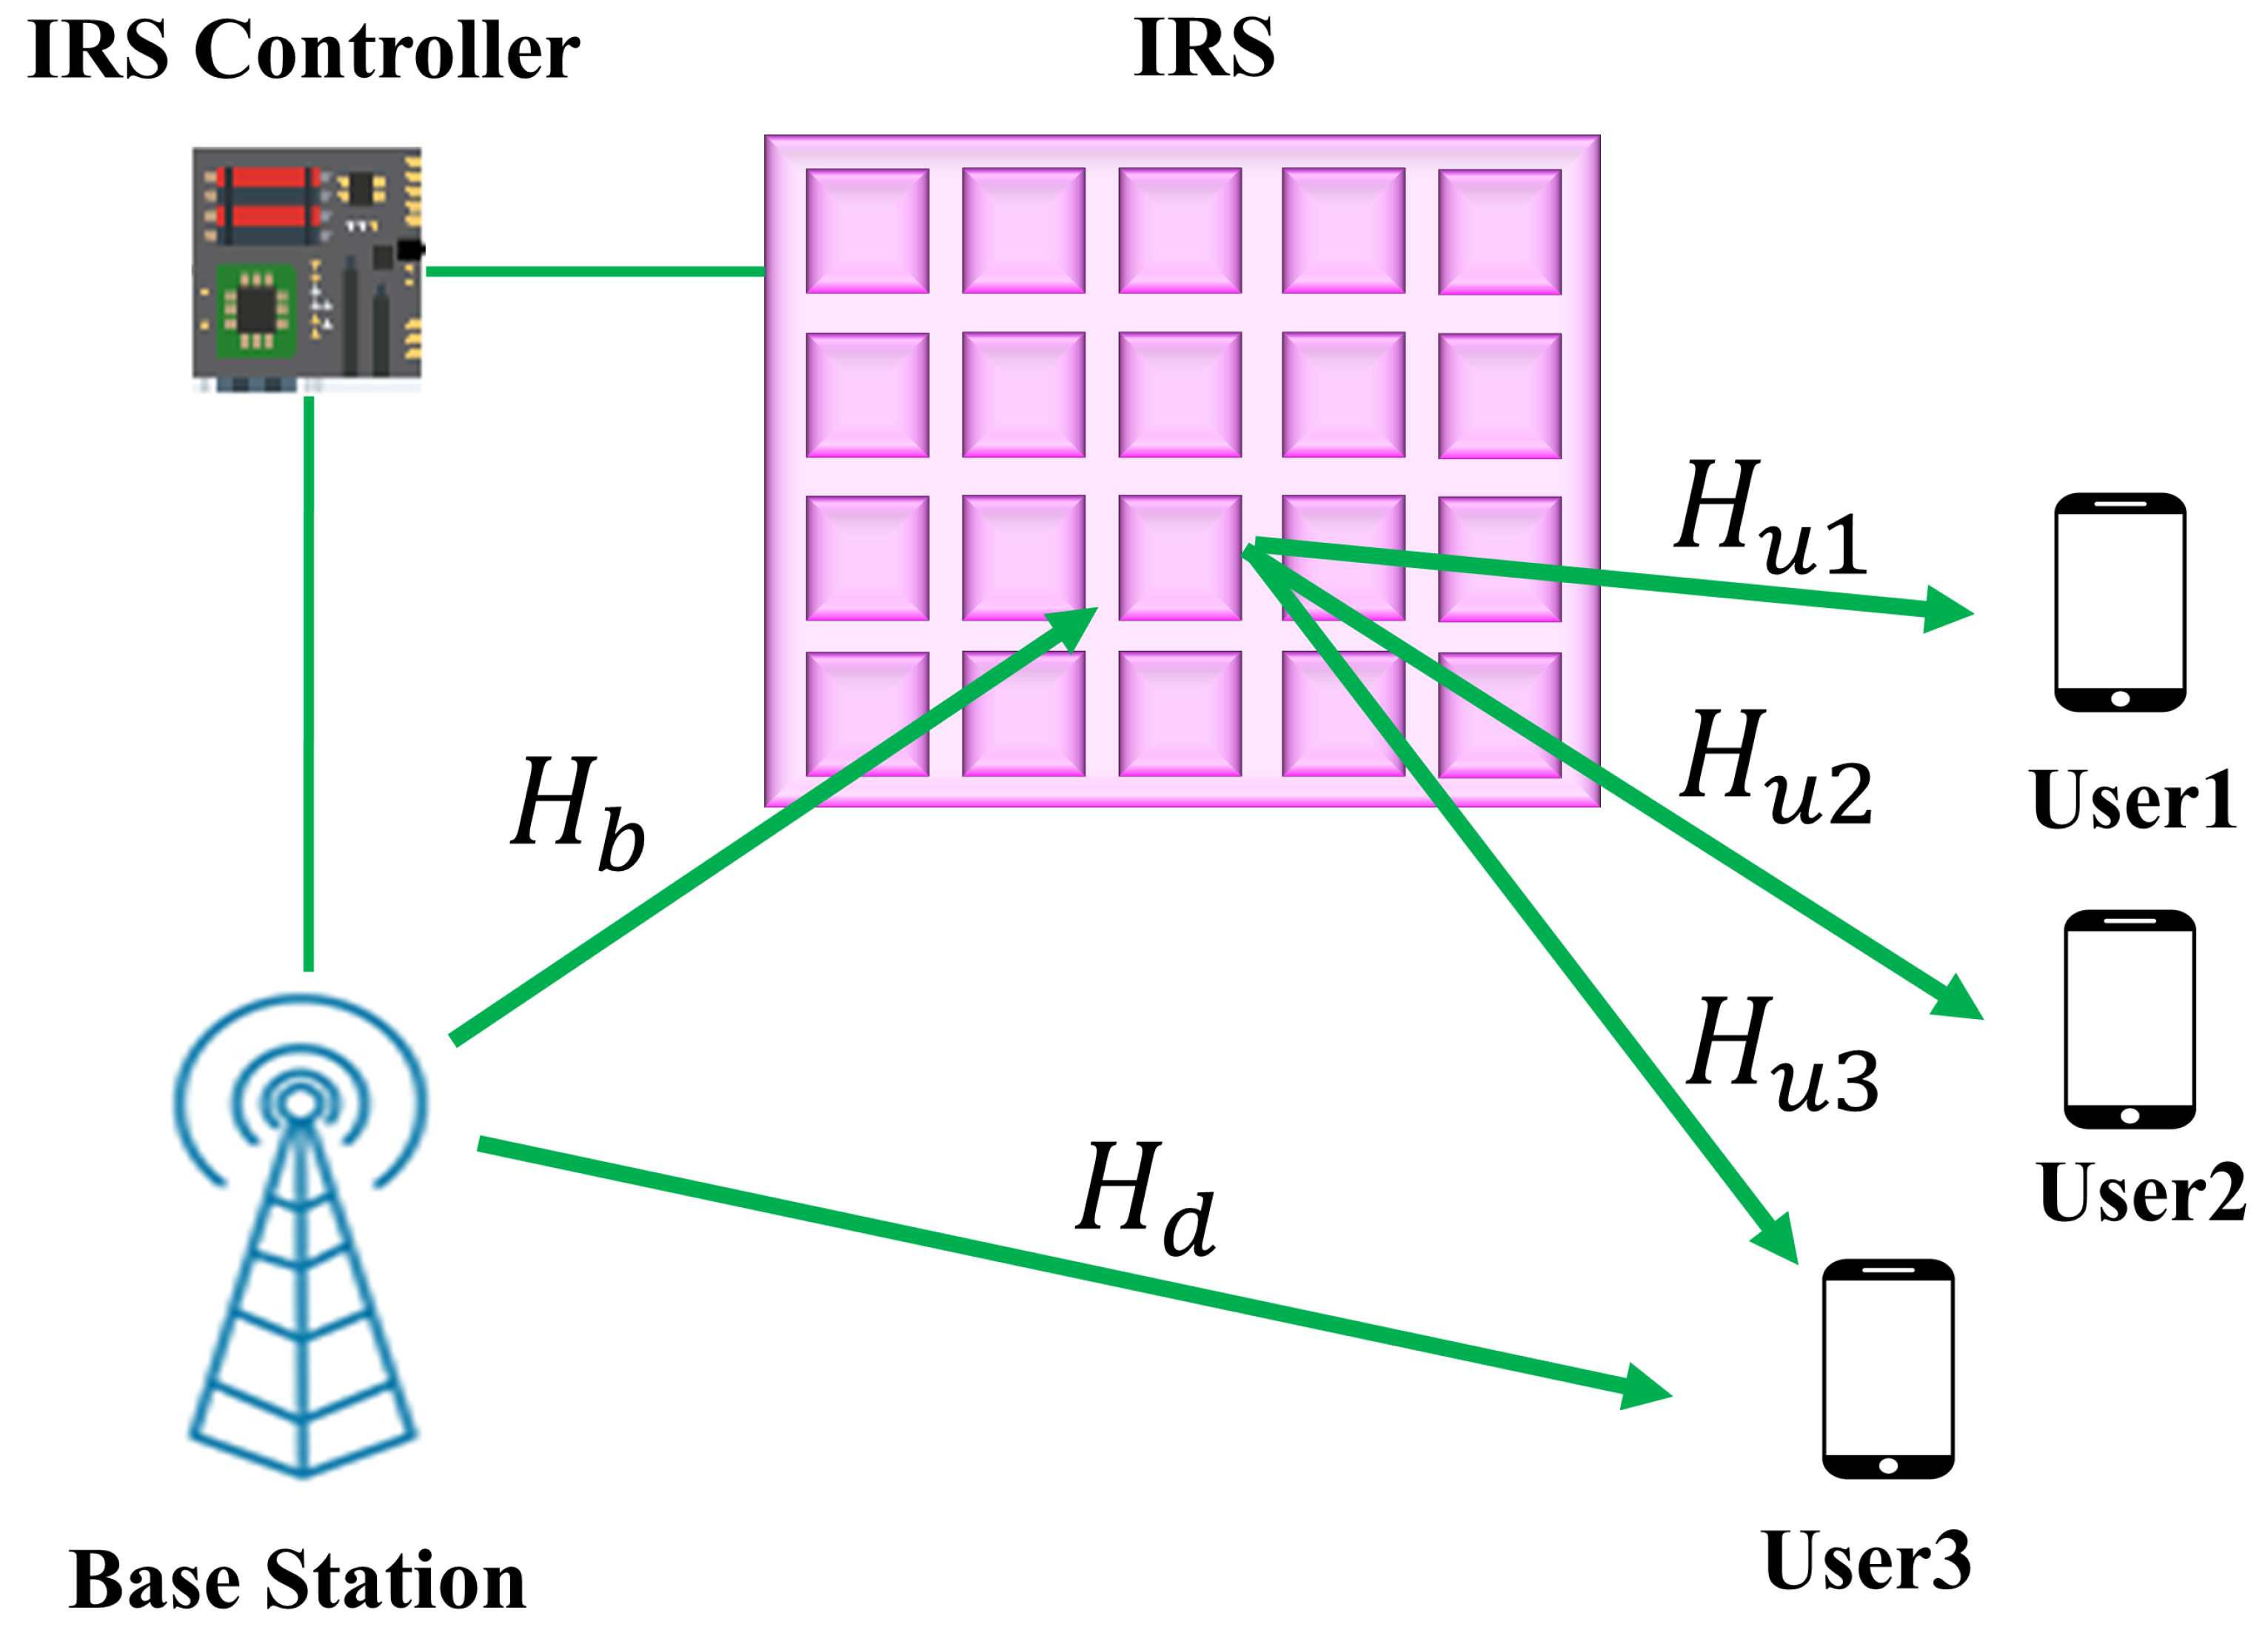
\includegraphics[width = 10cm, height = 6cm]{photo/2.4.2.png}
    \caption{Mô hình hoạt động của IRS}
    \label{Hình 6}
\end{figure}

Các bề mặt phản xạ không nhất thiết phải được chủ động đặt tại vị trí tính toán trước, mà có thể tận dụng các bề mặt có sẵn trong không gian như tường văn phòng, các tòa nhà trong thành phố,... để giảm thiểu chi phí lắp đặt mà vẫn đạt được mục tiêu truyền thông.\\

\begin{figure}[h!]
    \centering
    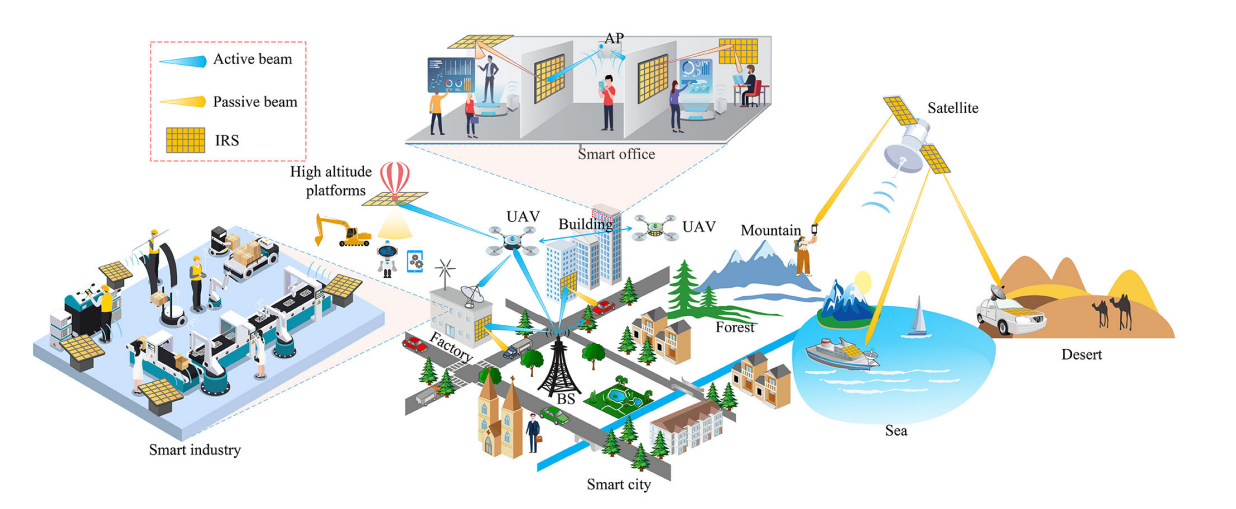
\includegraphics[width =15cm, height = 8cm]{photo/2.4.3.png}
    \caption{Minh họa ứng dụng của IRS trong các mạng không dây tương lai}
    \label{Hình 7}
\end{figure}


\paragraph{Ứng dụng của IRS}\\
\begin{itemize}

\item  Xây dựng hệ thống SIMO hoặc MIMO tại các khu vực có nhiều bề mặt phản xạ như trong thành phố hoặc văn phòng, tòa nhà,..\\
\begin{figure}[h!]
    \centering
    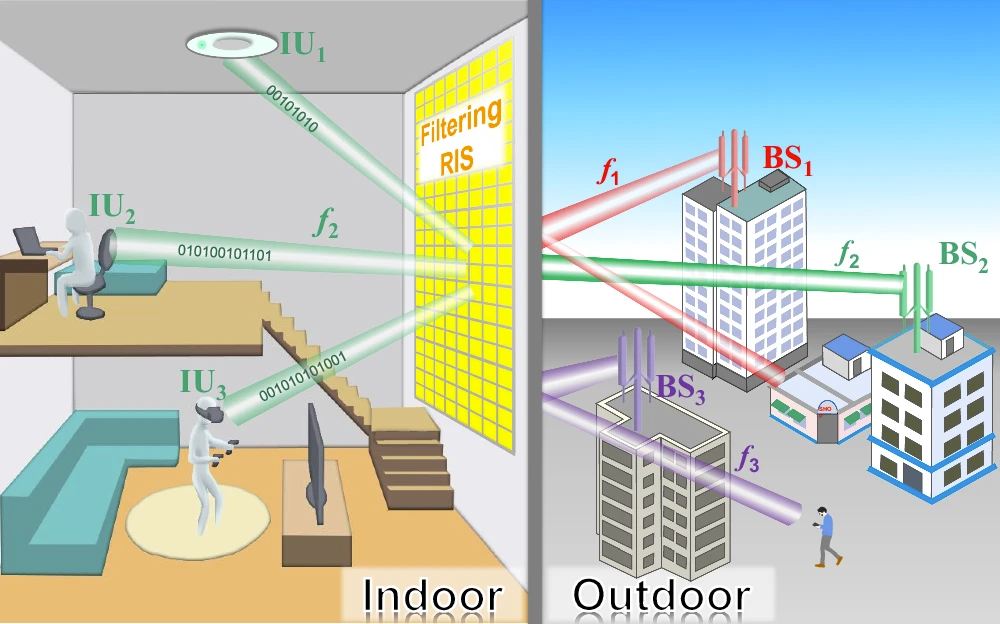
\includegraphics[width 12cm, height = 7cm]{photo/2.4.4.png}
    \caption{Không gian ứng dụng của IRS}
    \label{Hình 8}
\end{figure}

\item Tối ưu hóa tín hiệu trong không gian kín đã biết như tại hội trường, lớp học, rạp phim,..\\
\begin{figure}[h!]
    \centering
     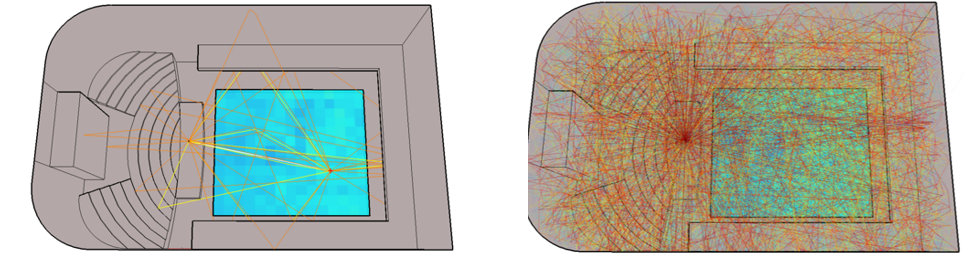
\includegraphics[width = 14cm, height = 6cm]{photo/2.4.5.png}
    \caption{Ứng dụng IRS trong môi trường kín}
    \label{Hình 9}
\end{figure}
\end{itemize}
\newpage
\paragraph{Ưu điểm và nhược điểm của IRS}
\subparagraph{Ưu điểm}
\begin{itemize}
    \item Tiết kiệm chi phí mở rộng: 
    Phương pháp bề mặt phản xạ thông minh giúp tiết kiệm chi phí khi cần mở rộng vùng phủ sóng vì chỉ cần lắp đặt mặt phản xạ tại một vị trí ta có thể sử dụng bộ điều khiển đề điều hướng tín hiệu đến nhiều vị trí mong muốn mà không cần triển khai thêm trạm phát, nhờ khả năng kiểm soát tín hiệu trong các môi trường có nhiều vật cản
    \item Hiệu quả năng lượng:
    Bề mặt phản xạ thông minh là một hệ thống thụ động, không tiêu tốn năng lượng để phát sóng mà chỉ phản xạ tín hiệu. Vì vậy, nó tiêu thụ rất ít năng lượng, phù hợp cho các ứng dụng yêu cầu tiết kiệm năng lượng.Bề mặt phản xạ thông minh giúp điều hướng tín hiệu hiệu quả hơn rất nhiều, phục vụ giảm nhiễu từ các thiết bị xung quanh và tăng cường cường độ tín hiệu đến máy thu
\end{itemize}
\subparagraph{Nhược điểm}
\begin{itemize}
    \item Khó khăn trong ước lượng kênh truyền: 
    Để IRS có thể phản xạ tín hiệu một cách tối ưu ta cần biết tương đối chính xách kênh truyền giữa máy phát và máy thu. Tuy nhiên, đây là một hệ thống vô cùng phức tạp để mô hình hóa toán học vì tín hiệu được phát đi, bên thu không chỉ thu được tín hiệu trực tiếp mà còn các bản sao khác nhau do môi trường tạo ra.
    \item Phức tạp trong điều khiển và tối ưu:
    IRS là một mô hình rất nhạy với điều kiện đầu vào, có thể xem như một hiệu ứng cánh bướm. Do đó, tín hiệu điều khiển phải đạt độ chính xác rất cao khi phát tín hiệu và khi điều khiển các phần tử của bề mặt phản xạ.
    \item Chi phí triển khai ban đầu:
    Mặc dù để mở rộng vùng phủ sóng, ta chỉ cần lắp thêm các bề mặt phản xạ và sẽ tối ưu chi phí hơn các trạm lặp lại, nhưng chi phí ban đầu để ước lượng và lắp đặt các bề mặt phản xạ trong một khu vực lớn thực sự là một thách thức lớn cho nhà đầu tư.
\end{itemize}

\subsubsection{Phương pháp dò tia - Ray Tracing}

Phương pháp dò tia trong ước lượng kênh truyền viễn thông là một kỹ thuật mô phỏng đường đi của sóng vô tuyến trong môi trường, nhằm hiểu rõ cách tín hiệu lan truyền từ máy phát đến máy thu qua các vật cản và điều kiện môi trường. Phương pháp dò tia đặc biệt hữu ích trong các hệ thống viễn thông có nhiều tín hiệu phản xạ, khúc xạ, tán xạ. Hay cụ thể hơn, phương pháp dò tia được ứng dụng để ước lượng kênh truyền sử dụng kỹ thuật bề mặt phản xạ thông minh. Để mô phỏng đường đi của các tín hiệu và xây dựng lại mô hình kênh truyền bằng phương pháp dò tia gồm các bước: Mô hình hóa môi trường truyền dẫn, tính toán đường truyền của tín hiệu (Ray Paths), uớc lượng tham số kênh và tổng hợp phản hồi xung kênh .\\

Mô hình hóa môi trường truyền dẫn cần phải xây dựng mô hình 3D của môi trường, bao gồm các vật cản như tường, trần, sàn nhà, và các cấu trúc khác. Các vật liệu và đặc tính của các vật cản này (như hệ số phản xạ, khúc xạ, hấp thụ) được gán giá trị tương ứng, giúp mô phỏng tín hiệu vô tuyến tương tác thực tế với môi trường. Việc mô hình hóa môi trường càng chi tiết giúp mô phỏng càng chính xác các hiện tượng ảnh hưởng đến tín hiệu, đặc biệt là trong các môi trường phức tạp như đô thị, tòa nhà lớn, hoặc khu vực nhiều vật cản.\\

\begin{figure}[h!]
    \centering
    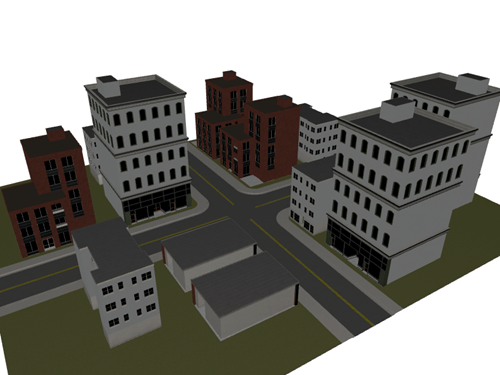
\includegraphics[width =10cm]{photo/2.4.6.png}
    \caption{Xây dựng mô hình 3D của môi trường}
    \label{Hình 10}
\end{figure}\\
Tính toán đường truyền của tín hiệu. Xem xét các loại đường truyền khác nhau của tín hiệu từ nguồn đến đích, bao gồm: Đường truyền trực tiếp giữa máy phát và máy thu, không gặp bất kỳ vật cản nào. Đường truyền tín hiệu bị phản xạ từ bề mặt của vật cản như tường hoặc trần nhà. Đường truyền khúc xạ khi tín hiệu đi qua các vật liệu như cửa kính, nó sẽ bị khúc xạ và thay đổi hướng. Đường truyền nhiễu xạ khi tín hiệu bị bẻ cong xung quanh các cạnh của vật thể. Ngoài ra ta cần phải xem xét về góc và độ trễ. Với mỗi loại đường truyền cần phải tính toán góc tới, góc phản xạ, và độ trễ của tín hiệu khi đi qua từng phần tử của môi trường. Những thông số này giúp xác định cách tín hiệu tới được điểm thu với các thành phần tín hiệu khác nhau.\\

Ước lượng tham số kênh. Sau khi xác định các đường truyền và các thành phần của tín hiệu đến máy thu, ta sẽ tiến hành ước lượng các tham số kênh quan trọng: Thời gian cần để tín hiệu di chuyển từ máy phát đến máy thu thông qua từng đường truyền. Góc đến xác định hướng mà tín hiệu tới bên thu thông qua các đường trực tiếp, phản xạ, khúc xạ, nhiễu xạ. Lượng năng lượng tín hiệu bị mất trong quá trình truyền qua môi trường. Từ các thông số đó, ứng dụng các phương pháp toán học phù hợp, ta sẽ tìm được ước lượng kênh truyền trong môi trường phức tạp bao gồm tín hiệu trực tiếp và các tín hiệu gián tiếp do môi trường tạo nên.\\
\newpage
Đối với phương pháp dò tia, sau khi đã xây dựng thành công môi trường cần truyền sóng truyền sóng và ước lượng được cách mà các tia phản xạ, khúc xạ sẽ di chuyển trong môi trường. Khi cần ước lượng kênh truyền giữa hai điểm bất kì trong không gian đã được mô hình hóa, ta sẽ không cần đến tín hiệu hoa tiêu để kiểm tra kênh truyền từ đó tiết kiệm được công suất cần để phát tín hiệu hoa tiêu. Với các tần số hoặc các mục tiêu cần lan truyền khác nhau, ta chỉ cần điều chỉnh hướng phát tín hiệu để đạt được mục đích mà không cần phải ước lượng nhiều kênh truyền cho nhiều đối tượng khác nhau. 

\begin{figure}[h!]
    \centering
  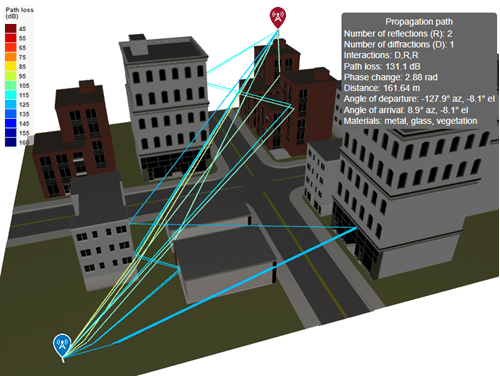
\includegraphics[width = 10cm]{photo/2.4.7.png}\\
    \caption{Ước lượng dò tia}
    \label{Hình 11}
\end{figure}

\subparagraph{Các thách thức đối với phương pháp dò tia}
\begin{itemize}

    \item  Chi Phí và khối lượng tính toán lớn:\\
    Phương pháp dò tia yêu cầu tính toán chi tiết các đường truyền của tín hiệu trong môi trường, bao gồm phản xạ, khúc xạ, và nhiễu xạ. Điều này đòi hỏi khả năng tính toán lớn, đặc biệt trong các môi trường phức tạp hoặc rộng lớn với nhiều vật cản.
    
    \item  Thời gian xử lý dài:\\
    Với yêu cầu tính toán nhiều đường truyền và các tham số liên quan, mô hình toán học của kênh truyền là vô cùng phức tạp và mất nhiều thời gian xử lý, khó đáp ứng trong các hệ thống yêu cầu ước lượng kênh thời gian thực.

    \item  Khó ước lượng trong các môi trường có sự thay đổi:\\
    Trong các môi trường có sự thay đổi liên tục như trong môi trường di động hoặc khi có nhiều vật thể di chuyển, phương pháp dò tia gặp khó khăn vì mô hình môi trường có thể thay đổi liên tục, dẫn đến các đường truyền và các tham số kênh thay đổi liên tục.

    \item  Yêu cầu nguồn dữ liệu đầu vào đáng tin cậy:\\
    Vì phương pháp rất nhạy với điều kiện đầu vào nên sẽ đòi hỏi dữ liệu chi tiết về môi trường, bao gồm bản đồ 3D, tính chất vật liệu và các yếu tố môi trường khác. Vì vậy, các bước thống kê ban đầu cần đạt độ chính xác cao để hệ thống hoạt động tốt.
\end{itemize}
\section{Mô hình ước lượng tham số ngõ vào đơn - ngõ ra đơn (Estimation Parameter in Single Input Single Output System - SISO)}

\subsection{Định nghĩa và mô hình SISO}

Trong hệ thống ngõ vào đơn - ngõ ra đơn (SISO), kênh có thể ảnh hưởng đến các tín hiệu có tần số khác nhau theo những cách khác nhau, vì vậy việc ước lượng kênh phải được thực hiện riêng cho từng kênh tần số. Tùy thuộc vào số lượng kênh, quá trình này có thể phức tạp và tiêu tốn nhiều tài nguyên. Do đó, thường thì việc ước lượng kênh chỉ được thực hiện cho một số kênh nhất định, và các ước lượng của những kênh còn lại sẽ được nội suy từ các ước lượng đã tính toán.\\

Mỗi kênh truyền đều được đặc trưng bởi một giá trị nhất định tại mỗi tần số cố định $(H)$. Tuy nhiên, giá trị mà cảm biến nhận được bên phía thu còn gồm cả phần nhiễu $(V)$ được mô tả như hình 1. Do đó, phương trình thực tế quan sát được bên phía thu có dạng \\
$$Y (observation) = H (parameter) + V (noise)$$

\begin{figure}[h!]
    \centering
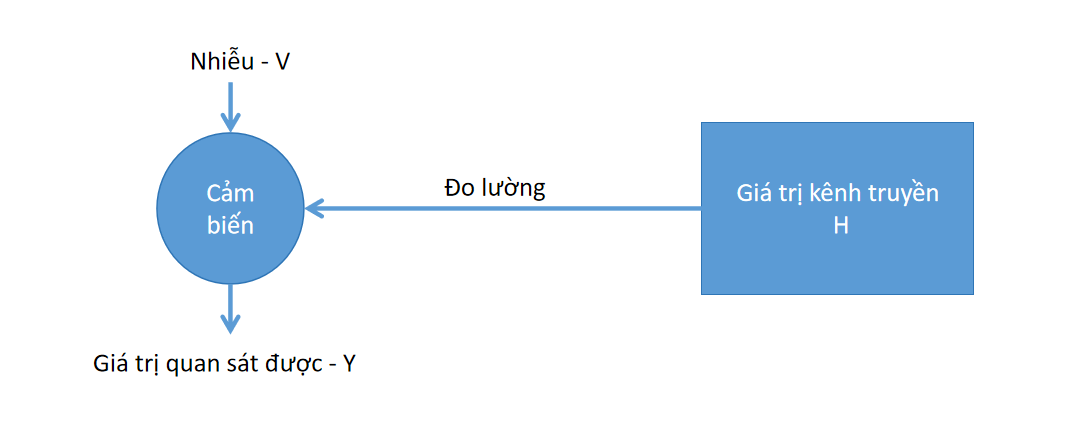
\includegraphics[width=15cm, height =6cm]{photo/3.1.1.png}
    \caption{Mô hình quan sát lý tưởng}
    \label{Hình 12}
\end{figure}

Với V là giá trị nhiễu, V là một biến ngẫu nhiên được đặc trưng bởi hàm mật độ xác suất có phân phối chuẩn với trung bình bằng không - $V \sim \mathcal{N}(0,\sigma^2)$. Vì vậy, Y cũng là một biến ngẫu nhiên\\
\[ E\{Y\} = E\{ H + V \}\ = E\{H\} + E\{V\}\]
$$ \text{Với } E\{H\} = H \text{, }  E\{V\} = 0 \text{ nên } E\{Y\} = H$$
\[\rightarrow E\{Y^2\} = E\{ (H + V)^2 \} \rightarrow E\{Y^2\} = \sigma^2 \] 

Vì vậy, ta có thể nói $Y$ là một biến ngẫu nhiên có phân phối chuẩn với trung bình là $H$ và phương sai $\sigma^2$. $Y \sim \mathcal{N}(H,\sigma^2)$. Từ đó, phương trình của biến ngẫu nhiên $Y$ có dạng hàm mật độ xác suất có dạng Gauss như sau:
$$F_y = \frac{1e^{\frac{-(Y-H)^2}{2\sigma^2}}}{\sqrt{2\pi\sigma^2}}$$

Trong phương trình của $F_y$, tham số $H$ là đại diện cho hàm truyền tại một tần số nhất định ta chưa biết giá trị. Nên việc cần làm ở đây là ước lượng tham số $H$ để tìm được kênh truyền tại các tần số khác nhau.

\subsection{Hàm hợp lý cực đại}
Do các tác động của nhiễu $V$ là ngẫu nhiên, nên các tín hiệu đo được $Y$ tại các thời điểm khác nhau cũng có giá trị khác nhau với mô tả là:
$$Y(1) = H + V(1)$$
$$Y(2) = H + V(2)$$
$$...$$
$$Y(N) = H + V(N)$$

Với $V(N) \sim \mathcal{N}(0,\sigma^2)$ và phương trình nhận được ở đầu thu được mô hình là $Y(k) = H + V(k)$ với $k$ là thời điểm đo. Dựa vào hàm mật độ xác suất của của $Y$. Ta tìm được hàm mật độ xác suất cho mỗi giá trị quan sát $Y(k)$ là:
$$F_{Y(k)} = \frac{1 e^{\frac{-(Y(k)-H)^2}{2\sigma^2}}}{\sqrt{2\pi\sigma^2}}$$

Do các biến $V(k)$ là độc lập nên giá trị quan sát $Y(k)$ cũng độc lập. Vì vậy hàm mật độ xác suất chung của quan sát sẽ là tích các hàm mật độ xác suất riêng lẽ:
$$F_{Y} = F_{Y(1)}\times F_{Y(2)}\times..F_{Y(N)}$$
$$P(\overline{Y}; H) = \frac{1 e^{\frac{-(Y(1)-H)^2}{2\sigma^2}}}{\sqrt{2\pi\sigma^2}} \times \frac{1 e^{\frac{-(Y(2)-H)^2}{2\sigma^2}}}{\sqrt{2\pi\sigma^2}} \times... \frac{1 e^{\frac{-(Y(N)-H)^2}{2\sigma^2}}}{\sqrt{2\pi\sigma^2}}$$


$$P(\overline{Y}; H)= {(\frac{1}{2 \pi \sigma^2})}^{\frac{N}{2}} e^{\sum_{k=1}^{N}{-\frac{1}{2 \sigma^2} (Y_k - H)^2}} $$

Trong phương trình của $F_Y$, tham số $H$ là tham số chưa biết. Tuy nhiên, phương trình $F_Y$ này có dạng giống như hàm đặc trưng của phương pháp ước lượng hợp lý cực đại (Maximum Likelihood Estimate - ML). Từ lý thuyết của ML ta có $ P(\overline{Y}; H)$ với $\overline{Y}$ là giá trị trung bình của các quan sát được viết dưới dạng vector $\overline{Y}^T = [Y(1), Y(2),...Y(N)]$. Hàm này mô tả mật độ xác suất chung của các quan sát $Y(1), Y(2),..Y(N)$ được tham số hóa bởi $H$ được sử dụng để tìm giá trị của $H$ mà làm cho hàm khả năng đạt cực đại - hay ước lượng khả năng xảy ra lớn nhất.\\

Bây giờ, ta sẽ tìm điều kiện để hàm $ P(\overline{Y}; H)$ đạt cực đại đồng nghĩa với tìm $H$ hợp lý nhất bằng cách lấy logarithm để dễ dàng tính toán:
$$\ln P(\overline{Y}; H) = \ln {(\frac{1}{2 \pi \sigma^2})}^{\frac{N}{2}} e^{\sum_{k=1}^{N}{-\frac{1}{2 \sigma^2} (Y_k - H)^2}} $$
$$\ln P(\overline{Y}; H) =\frac{-N}{2} \ln2\pi\sigma^2 - \frac{1}{2\sigma^2} \sum_{k=1}^{N}(Y(k)-H)^2$$

Ta sẽ tối ưu hóa hàm hợp lý (likelihood functinon) để tìm ước lượng hợp lý cực đại của tham số $H$. Để làm việc này ta cần tối ưu biểu thức $\sum_{k=1}^{N}(Y(k)-H)^2$ bằng cách lấy đạo hàm theo biến $H$ và cho bằng không. Ta tìm được giá trị của $H$ mà tại đó hàm hợp lý đạt cực đại gọi là $\hat{H}$. Hay nói cách khác $\hat{H}$ là giá trị kênh truyền cần tìm hợp lý nhất\\
$$\frac{\partial}{\partial H} \sum_{k=1}^{N}(Y(k)-H)^2 = 0$$
$$ \rightarrow \sum_{k=1}^{N}2(Y(k)-H) = 0$$ 
$$ \rightarrow \sum_{k=1}^{N}Y(k) = NH$$
$$ \hat{H} = \frac{1}{N}\sum_{k=1}^{N}Y(k) $$
\subsection{Các đặc tính của ước lượng hợp lý cực đại - Properties of Maximum Likelihood Estimate }
Từ phương trình của $\hat{H}$ ta có thể thấy nó phụ thuộc vào giá trị trung bình của $Y(k)$. Tuy nhiên $Y(k)$ là như đã chứng minh là một biến ngẫu nhiên phân phối chuẩn $Y \sim \mathcal{N}(H,\sigma^2)$. Nên giá trị ước tính của $\hat{H}$ cũng là giá trị ngẫu nhiên phân phối chuẩn trong thực tế. Vì vậy, giá trị $\Hat{H}$ không phải là giá trị $H$ chính xác mà chỉ là một ước lượng và vẫn bị ảnh hưởng bởi nhiễu.
$$\hat{H} = \frac{\sum_{k=1}^{N}Y(k)}{N} \text{ với }Y(k) = H + V(k) $$
$$\hat{H} = \frac{NH + \sum_{k=1}^{N}V(k) }{N}$$
$$\hat{H} = H + \frac{1}{N} \sum_{k=1}^{N}V(k) \rightarrow \hat{H} \neq H$$

Để tìm được giá trị $H$ chính xác, ta cần xem xét các hành vi của $\hat{H}$ về trung bình, phương sai và làm thế nào để ước lượng $\hat{H}$ tiến gần đến giá trị $H$ chính xác.
\[ E\{\hat{H}\} = E\{H + \frac{1}{N}\sum_{k=1}^{N}V(k)\}\ \]
$$ E\{\hat{H}\} = E\{H\} + E\{\frac{1}{N}\sum_{k=1}^{N}V(k)\}$$
$$ E\{\hat{H}\} = H + 0 = H $$

Ta có thể thấy, trung bình của các ước lượng bằng với giá trị thực tế của tham số $H$, $\hat{H} = H$. Và ước lượng này là một ước lượng không chệch, nghĩa là giá trị trung bình của ước lượng bằng với giá trị thực của tham số. Và do $\hat{H}$ là một biến phụ thuộc vào tổng các biến ngẫu nhiên có phân phối chuẩn $Y \sim \mathcal{N}(H,\sigma^2)$ nên $\hat{H}$ cũng là một biến ngẫu nhiên có phân phối chuẩn với trung bình là $H$. Và với một biến ngẫu nhiên có phân phối chuẩn, ta cần quan tâm đến phương sai của $\hat{H}$.

$$E\{ (\hat{H} - E\{\hat{H}\})^2 \} = E\{ (\hat{H} - H)^2 \}$$

$$ \text{mà } \hat{H} = H + \frac{1}{N} \sum_{k=1}^{N}V(k) \text{ nên }  \hat{H} - H = \frac{1}{N} \sum_{k=1}^{N}V(k)$$ 
$$ \rightarrow E\{ (\hat{H} - E\{\hat{H}\})^2 \} = E \{ ( \frac{1}{N} \sum_{k=1}^{N}V(k) )^2 \}  $$
$$E\{ (\hat{H} - E\{\hat{H}\})^2 \} = \frac{1}{N^2} E\{ ( \sum_{k=1}^{N}V(k)) ( \sum_{l=1}^{N}V(l)) \}$$
$$E\{ (\hat{H} - E\{\hat{H}\})^2 \} = \frac{1}{N^2} E\{ ( \sum_{k=1}^{N} \sum_{l=1}^{N}V(l)V(k)) \}$$
$$E\{ (\hat{H} - E\{\hat{H}\})^2 \} = \frac{1}{N^2} \sum_{k=1}^{N} \sum_{l=1}^{N}   E\{ V(l)V(k) \}$$

Nhắc lại về nhiễu, nhiễu là một biến ngẫu nhiên độc lập có phân phối chuẩn. Vì vậy ở đây $V(k)$ và $V(l)$ đều là các biến ngẫu nhiên độc lập với nhau nên.

$$E\{ V(l)V(k) \} = E \{ V(l)\} E\{V(k)\}$$
Ứng dụng lý thuyết xác suất về các biến ngẫu nhiên không tương quan (uncorrelated) ta có kết quả sau:

$$E \{V(l)\} E\{V(k)\} = \begin{cases} 
0 & \text{nếu } k \neq l \\
E \{ V^2(k) \} = \sigma^2 & \text{nếu } k = l $$
\end{cases}

$$E \{ V(l)\} E\{V(k)\} = \sigma^2 \delta(k-l)$$
$$ \rightarrow E\{ (\hat{H} - E\{\hat{H}\})^2 \} = \frac{1}{N^2} \sum_{k=1}^{N} \sum_{l=1}^{N} \sigma^2 \delta(k-l) = \frac{1}{N^2} \sum_{k=1}^{N} \sigma^2 \delta(k-l)  = \frac{N\sigma^2}{N^2} = \frac{\sigma^2}{N} $$

Ta có thể thấy, phương sai của ước lượng cho kênh truyền là $\frac{\sigma^2}{N}$. Và $\sigma^2$ cũng là phương sai của công suất nhiễu ngẫu nhiên $V(k)$. Vì vậy ta có thể nói rằng, nếu các nhiễu ngẫu nhiên $V(k)$ là biến ngẫu nhiên độc lập với $V \sim \mathcal{N}(0,\sigma^2)$ thì ước lượng kênh chuyền theo phương pháp ước lượng hợp lý cực đại sẽ là một ước lượng không chệch với giá trị trung bình của ước lượng $\hat{H}$ sẽ bằng với giá trị chính xác $H$ và phương sai của ước lượng là $\frac{\sigma^2}{N}$ - phương sai của nhiễu $\sigma$ chia cho số mẫu được thử nghiệm $N$ $\frac{\sigma^2}{N}$.

Dựa vào kết quả vừa chứng minh được ta có $\hat{H} \sim \mathcal{N}(H,\frac{\sigma^2}{N})$ và lý thuyết phân phối xác xuất (hình 2). Số mẫu thử nghiệm $N$ sẽ ảnh hưởng đến kết quả của ước lượng theo mô hình nghịch biến, số mẫu càng ít ước lượng càng không đáng tin do phương sai tăng lên, ngược lại ước lượng sẽ càng tiến về giá trị trung bình khi $N$ càng lớn và ước lượng $\hat{H}$ sẽ đúng bằng giá trị $H$ cần tìm khi $N = \infty$

\begin{figure}[h!]
    \centering
    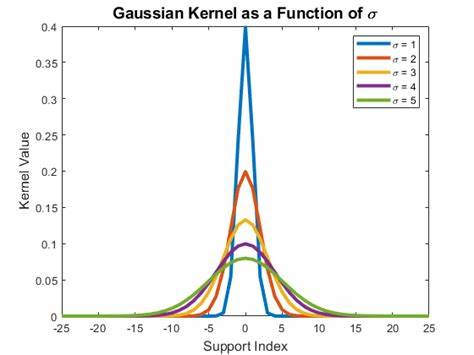
\includegraphics[width=12cm, height =7cm]{photo/3.3.1.png}
    \caption{ô hình phân phối xác suất theo $\sigma$}
    \label{Hình 13}
\end{figure}
\subsection{Tối ưu hóa độ tin cậy và số mẫu thử cần thiết  - Reliability of the Estimation \& Number of Samples Required}
Như đã kết luận ở phần 2.2 về đặc trưng của $\hat{H}$ cụ thể là $\hat{H} \sim \mathcal{N}(H,\frac{\sigma^2}{N})$. Độ tin cậy của ước lượng sẽ càng chính xác khi các mẫu thử $N$ tiến đến vô cùng. Trong thực tế việc thử với vô cùng mẫu là không khả thi và gây tốn kém, vì vậy ta cần tìm giá trị $N$ phù hợp để đáp ứng được độ tin cậy để ước lượng phải đủ để có thể sử dụng và số mẫu phải tối thiểu để giảm được thời gian và chi phí thử nghiệm. Cụ thể ta cần tìm $N$ để xác suất mà ước lượng $\hat{H}$ nằm trong khoảng $\frac{\sigma}{2}$ của giá trị chính xác $H$ là $\geq 99.99\%$. Đầu tiên ta sẽ tìm $N$ để độ tin cậy của ước lượng là $99.99\%$

$$P(\|\hat{h} - h\| \leq \frac{\sigma}{2}) \geq 0.9999$$
$$P(\|\hat{h} - h\| \geq \frac{\sigma}{2}) \leq 1 - 0.9999 = 0.00001$$
$$ \text{Gọi W là sai số ước lượng: } W = \hat{H} - H $$

$$\rightarrow P(\|W\| \geq \frac{\sigma}{2}) \leq 0.00001$$
$$\rightarrow P(W \geq \frac{\sigma}{2}) + P(W \leq \frac{-\sigma}{2}) \leq 0.00001$$
$$W = \hat{H} - H \text{ mà } \hat{H} \sim \mathcal{N}(H,\frac{\sigma^2}{N}) \rightarrow W \sim \mathcal{N}(0,\frac{\sigma^2}{N})$$
$$\text{Vì vậy: } F_W(W) = \frac{1}{ \sqrt{2\pi\frac{\sigma^2}{N} } } e^\frac{-NW^2}{2\sigma^2}$$

$$ \rightarrow \int_{\frac{\sigma^2}{2}}^{+\infty} F_w(w)dw + \int_{-\infty}^{\frac{-\sigma^2}{2}} F_w(w)dw \leq 0.00001$$
$$\text{do } F_w(w) = F_w(-w) \rightarrow 2\int_{\frac{\sigma^2}{2}}^{+\infty} F_w(w)dW \leq 0.00001$$
$$\int_{\frac{\sigma^2}{2}}^{+\infty} F_w(w)dW  = \int_{\frac{\sigma^2}{2}}^{+\infty}\frac{1}{ \sqrt{2\pi\frac{\sigma^2}{N} } } e^\frac{-NW^2}{2\sigma^2} \leq 0.00005$$
$$\text{Đặt: } \frac{W^2}{\frac{\sigma^2}{N}} = t^2 = \frac{NW^2}{\sigma^2} \rightarrow W = \frac{\sigma t}{\sqrt{N}} \text{ Suy ra } dW = \frac{\sigma dt}{\sqrt{N}}$$
$$\rightarrow \int_{\frac{\sigma^2}{2}}^{+\infty}\frac{1}{ \sqrt{2\pi\frac{\sigma^2}{N} } } e^\frac{-NW^2}{2\sigma^2} = \int_{\frac{\sqrt{N}}{2}}^{+\infty}\frac{1}{ \sqrt{2\pi\frac{\sigma^2}{N} } } e^\frac{-t}{2} \frac{\sigma}{\sqrt{N}} \leq 0.00005 $$

$$ \rightarrow \int_{\frac{\sqrt{N}}{2}}^{+\infty}\frac{1}{ \sqrt{2\pi}} e^\frac{-t}{2} dt \leq 0.00005 $$

Hàm mật độ xác suất này có dạng $\mathcal{N} (0,1)$, do đó tích phân này có thể xem như một tích phân để tìm xác suất của một biến ngẫu nhiên có phân phối chuẩn.
$$Q(x) = \int_{\frac{\sqrt{N}}{2}}^{+\infty}\frac{1}{x} e^\frac{-t}{2} dt = Pr(T \geq x) \rightarrow Q(\frac{\sqrt{N}}{2}) \leq 0.00005$$
$$\rightarrow \frac{\sqrt{N}}{2} \geq Q^{-1} (0.0005) = 60.54$$
$$  \rightarrow N =61$$

Tiếp theo, ta sẽ tìm $N$ để giá trị ước lượng $\hat{H}$ nằm trong khoảng $(+\frac{\sigma}{2};-\frac{\sigma}{2})$. Dựa vào tính chất của phân phối chuẩn ta có hàm $Q(x)$ là xác suất xuất hiện của hàm biến ngẫu nhiên $x$ với trung bình là $0$ và phương sai là $1$ phù hợp với mô hình ước lượng số lượng mẫu $N$ ta đang xét. Xấp xĩ hàm $Q(x)$ khi $X \sim \mathcal{N}(0,1)$. Sau đó sẽ đổi biến $x=\frac{\sqrt{N}}{2}$ để phù hợp với mô hình tìm $N$ ta được.
$$Q(x) \approx \frac{1}{2} e^{-\frac{1}{2} x^2}$$
$$\rightarrow Q(\frac{\sqrt{N}}{2}) \approx \frac{1}{2}e^{-\frac{1}{2}\frac{N}{4}} \leq 0.00005$$
$$\rightarrow -\frac{N}{8} \leq ln(0.0001)$$
$$N \geq -8ln(0.0001) = 73.68$$
$$\rightarrow N \geq 74$$

Với kết quả như trên, bằng các lý thuyết xác suất và tính chất của phân phối chuẩn. Ta đã tìm được giá trị của số lượng mẫu thử $N$ để giá trị của ước lượng kênh truyền được tối ưu hóa cho phù hợp với yêu cầu đưa ra ban đầu là tìm $N$ để xác suất mà ước lượng $\hat{H}$ nằm trong khoảng $\frac{\sigma}{2}$ của giá trị chính xác $H$ là $\geq 99.99\%$
\subsection{Ước lượng tham số phức - Estimation of Complex Parameters}

Dựa vào các mô hình ước lượng tham số thực để có thể mở rộng và ước lượng cho một tham số phức. 
$$\text{Tham số phức có dạng: }h (complex) = h_R (\text{real part}) + jh_I (\text{imaginary part})$$
$$\text{Ta có mô hình tham số thực: } y(k) = h + v(k)$$
$$y_R(k) + jy_I(k) = (h_R + jh_I) + (V_R(k) + j V_I(k))$$
$$\text{(complex observation)  }  \text{ (complex parameter) }  \text{ (complex noise})$$

Với mô hình tham số phức, mọi tham số có mặt ta đều xét là một số phức $a+jb$. Nên giá trị tham số có dạng $h_R + jh_I$, nhiễu có dạng $v_R(k) + j v_I(k)$. Giá trị quan sát $y$ là tổng của hai số phức, vì vậy $y$ cũng là một số phức $y_R(k) + jy_I(k)$. Bằng cách sử dụng tính chất của số phức, ta có thể chia một số phức hai thành: phần thực và phần ảo. Sau đó áp dụng tương tự các ước lượng như với tham số thực để chuyển từ một phép ước lượng khó thành hai ước lượng phần thực riêng và phần ảo riêng dễ thực hiện hơn. \\

Phần thực:
$$y_R(1) = h_R + v_R(1)$$
$$y_R(2) = h_R + v_R(2)$$
$$\text{...}$$
$$y_R(N) = h_R + v_R(N)$$
$$\rightarrow \text{ước lượng phần thực: }\hat{h}_R = \frac{1}{N}\[
\sum_{k=1}^{N} y_R(k) \]$$

Phần ảo:
$$y_I(1) = h_I + v_I(1)$$
$$y_I(2) = h_I + v_I(2)$$
$$\text{...}$$
$$y_I(N) = h_I + v_I(N)$$
$$\rightarrow \text{ước lượng phần ảo: }\hat{h}_I = \frac{1}{N}\[
\sum_{k=1}^{N} y_I(k) \]$$

Kết quả ước lượng tham số phức sau khi ước lượng hai thành phần là: $\hat{h} = \hat{h}_R + j\hat{h}_I$
\subsection{Các đặc tính của tham số phức - Properties of the Complex Parameter}
$$ \text{Ta có: }V(k) = V_R(k) + j V_I(k)$$

Giả sử rằng: $V_R(k) \text{ tuân theo phân phối chuẩn với trung bình là 0, phương sai là }\frac{\sigma^2}{2}$: $V_R(k) \sim\mathcal{N}(0,\frac{\sigma^2}{2})$. $V_I(k) \text{ tuân theo phân phối chuẩn với trung bình là 0, phương sai là } \frac{\sigma^2}{2}$: $V_I(k) \sim \mathcal{N}(0,\frac{\sigma^2}{2})$. \text{Ngoài ra,} $V_R(k)$ và $jV_i(k)$ là biến ngẫu nhiên và không tương quan với nhau. Vì vậy, ta gọi $V_R(k)$ và $jV_i(k)$ là nhiễu Gaussian với trung bình là không và có tính đối xứng. Hay ta có thể viết.
$$ E\{V_R(k)V_I(K)\} = E\{V_R(k)\}E\{V_I(K)\} = 0 $$
$$ E\{V(k)\} = E\{V_R(k)\}+jE\{V_I(K)\} = 0 + j0 = 0$$
$$ E\{\|V(k)\|^2\} = E\{\|V_R(k)\|^2\}+E\{\|V_I(K)\|^2\} = \frac{\sigma^2}{2} + \frac{\sigma^2}{2} = \sigma^2$$
Hay có thể nói rằng, phần thực của nhiễu chiếm một nữa công suất, phần ảo của nhiễu chiếm một nữa công suất. Dựa vào các tính chất ở trên, ta sẽ lần lượt tìm các đặc tính và hành vi của ước lượng $\hat{H}$ hay cụ thể hơn là các thành phần phần thực và phần ảo của $\hat{h}$ như sau:\\

Với phần thực:
$$\hat{h}_R = \frac{1}{N} \sum_{k=1}^{N} y_R(k) \text{ với } y_R(k) = h_R + v_R(k)$$
$$\text{Tương tự như phần 2.3} \rightarrow \hat{h}_R = h_R + \frac{1}{N} \sum_{k=1}^{N} v_R(k) \text{ và } \begin{cases}
   E\{\hat{h_R}\} = h_R &\\
   E\{\|\hat{h_R}-h_R\|^2\} = \frac{1}{N}\frac{\sigma^2}{2} = \frac{\sigma^2}{2N}&
\end{cases}$$

Với phần ảo:
$$\hat{h}_I = \frac{1}{N} \sum_{k=1}^{N} y_I(k) \text{ với } y_R(k) = h_I + v_I(k)$$
$$\text{Tương tự như phần 2.3} \rightarrow \hat{h}_I = h_I + \frac{1}{N} \sum_{k=1}^{N} v_I(k) \text{ và } \begin{cases}
   E\{\hat{h_I}\} = h_I &\\
   E\{\|\hat{h_I}-h_I\|^2\} = \frac{1}{N}\frac{\sigma^2}{2} = \frac{\sigma^2}{2N}&
\end{cases}$$

%Sai số của ước lượng: $W = W_R + jW_I$ 
$$ \text{Sai số của ước lượng: } W = W_R + jW_I \text{ với } \begin{cases}
    W_R = \frac{1}{N} \sum_{k=1}^{N} v_R(k) &\\
    W_I = \frac{1}{N} \sum_{k=1}^{N} v_I(k)
\end{cases}$$
Bởi vì $V_R(k) \sim \mathcal{N}(0,\frac{\sigma^2}{2})$ và $V_I(k) \sim \mathcal{N}(0,\frac{\sigma^2}{2})$ hai biến ngẫu nhiên này độc lập, không tương quan nhau ở đa số các trường hợp trên thực tế nên sai số ước lượng $W_R$ và $W_I$ cũng độc lập và không tương quan.
$$ E\{W_R(k)W_I(K)\} = E\{W_R(k)\}E\{W_I(K)\} = 0 $$
\section{Ước lượng kênh truyền ngõ vào đơn - ngõ ra đơn}
\subsection{Mô hình kênh truyền tuyến tính bất biến}

Trong báo cáo này giả sử kênh truyền là tuyến tính bất biến (LTI) để phù hợp với các lý thuyết và dễ dàng thực hiện. Giá trị kênh truyền trên thực tế là không thể biết chính xác nhưng có thể ước lượng được, vì vậy chúng ta cần phải ước lượng kênh truyền giữa các đơn vị truyền nhận tín hiệu để đưa ra các giải pháp tối ưu khi thiết kế hệ thống viễn thông. Mô hình kênh truyền SISO gồm một bên phát và một bên nhận. Bên phát gửi tín hiệu qua kênh truyền và bên nhận thu được tín hiệu bao gồm tín hiệu phát, độ suy hao của kênh truyền và nhiễu
$$y(k) = h.x(k) + v(k)$$
$$\text{(Quan sát) = (kênh truyền).(tín hiệu phát) + (nhiễu)}$$

\begin{figure}[h!]
    \centering
     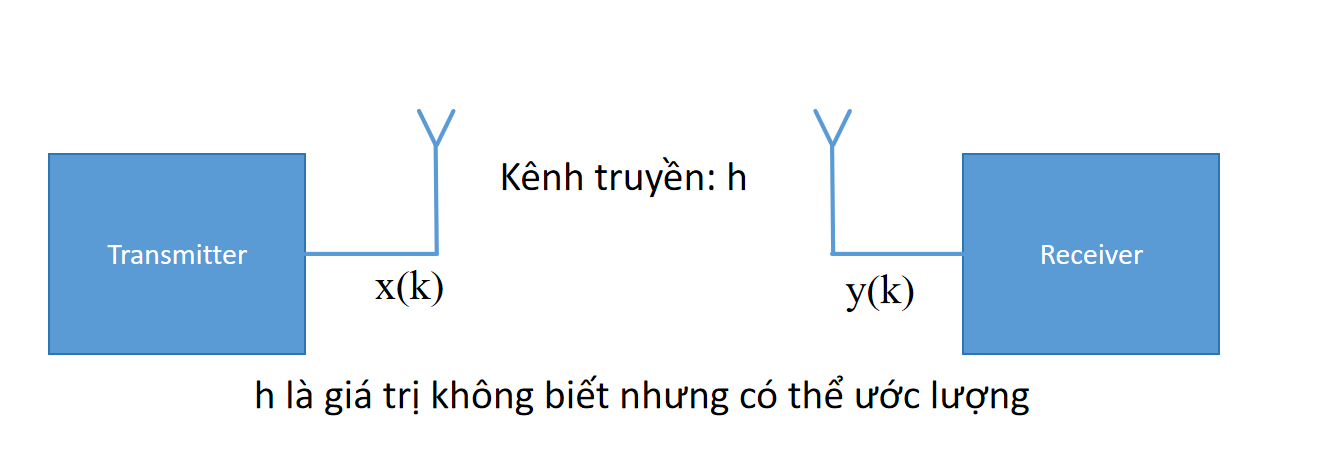
\includegraphics[width=14cm, height =6cm]{photo/4.1.1.png}
    \caption{Mô hình truyền nhận tín hiệu}
    \label{Hình 14}
\end{figure}

Phương pháp ước lượng như sau. Bên phát sẽ phát đi các tín hiệu hoa tiêu đã biết để thử nghiệm, các tín hiệu hoa tiêu sau khi bị ảnh hưởng bới kênh truyền và nhiễu sẽ đến được với bên thu. Khi bên thu nhận được tín hiệu sẽ tiến hành giải mã. Dựa vào tín hiệu hoa tiêu phát đi và tín hiệu thu được bằng các biến đổi toán học, mô hình hóa ta sẽ ước lượng được giá trị của kênh truyền. Để thực hiện ta ký hiệu như sau:
$$\text{Tín hiệu hoa tiêu: } x(1), x(2), x(3),...x(N)$$
$$\text{Tín hiệu thu: } y(1), y(2), y(3),...y(N)$$
Mô hình truyền nhận tín hiệu:
$$y(1) = h.x(1) + v(1) $$
$$y(2) = h.x(2) + v(2)$$
$$y(3) = h.x(3) + v(3)$$
$$...$$
$$y(N) = h.x(N) + v(N)$$
$$\rightarrow \overline{Y} = h.\overline{X} + \overline{V}$$
\subsection{Đưa mô hình kênh truyền về lý thuyết xác suất}
Tương tự như phần ước lượng tham số, chúng ta sẽ giả sử rằng các nhiễu tác động lên kênh truyền là biến ngẫu nhiên có phân phối chuẩn và độc lập, không tương quan với nhau nên các tín hiệu $y(k)$ quan sát được cũng là độc lập. Do đó hàm phân phối xác suất của $y$ là tích xác suất xuất hiện của các quan sát $y(k)$ thành phần
$$V(k) \sim \mathcal{N}(0,\sigma^2) \rightarrow Y(k) \sim \mathcal{N}(h.x(k),\sigma^2)  \rightarrow F_Y(K)(y(k)) = \frac{1}{\sqrt{2\pi\sigma^2}} e^{-\frac{1}{2\sigma^2} (y(k) - x(k))^2} $$

$$F_{Y(1)Y(2)...Y(N)}(y(1)y(2)...y(N)) = F_{Y(1)}y(1)\times F_{Y(2)}y(2)\times..F_{Y(N)}y(N)$$

Ta có thể thấy, hàm phân phối xác suất của $Y$ là một hàm số có tham số ẩn là $h$. Đây là hàm hợp lý theo biến $h$
$$P(\overline{Y}; H) = \frac{1 e^{\frac{-(Y(1)-H.x(1))^2}{2\sigma^2}}}{\sqrt{2\pi\sigma^2}} \times \frac{1 e^{\frac{-(Y(2)-Hx(2))^2}{2\sigma^2}}}{\sqrt{2\pi\sigma^2}} \times... \frac{1 e^{\frac{-(Y(N)-H.x(N))^2}{2\sigma^2}}}{\sqrt{2\pi\sigma^2}}$$

$$P(\overline{Y}; H)= {(\frac{1}{2 \pi \sigma^2})}^{\frac{N}{2}} e^{\sum_{k=1}^{N}{-\frac{1}{2 \sigma^2} (Y(k) - H.x(k))^2}} $$

Bây giờ, ta sẽ tìm điều kiện để hàm $ P(\overline{Y}; H)$ đạt cực đại đồng nghĩa với tìm $H$ hợp lý nhất bằng cách lấy logarithm để dễ dàng tính toán sau đó tìm đạo hàm của hàm hợp lý và cho bằng không:
$$\ln P(\overline{Y}; H) = \ln {(\frac{1}{2 \pi \sigma^2})}^{\frac{N}{2}} e^{\sum_{k=1}^{N}{-\frac{1}{2 \sigma^2} (Y_k - h.x(k))^2}} $$
$$\ln P(\overline{Y}; H) =\frac{-N}{2} \ln2\pi\sigma^2 - \frac{1}{2\sigma^2} \sum_{k=1}^{N}(Y(k)-h.x(k))^2$$

$$\frac{\partial ln(P(\overline{Y};h))}{\partial h} = -\frac{1}{2\sigma^2} \sum_{k=1}^{N} 2(y(k) - h.x(k)).(-x(k)) = 0$$
$$ \rightarrow \sum_{k=1}^{N} (y(k) - h.x(k)).x(k) = 0$$
$$\rightarrow \sum_{k=1}^{N} x(k)y(k) = h\sum_{k=1}^{N} x^2(k)$$
$$\rightarrow \hat{h} = \frac{\sum_{k=1}^{N} x(k)y(k)}{\sum_{k=1}^{N} x^2(k)} \text{ Đây là giá trị ước lượng của }h$$

Dựa vào kết quả vừa chứng minh, có thể nhận xét rằng giá trị ước lượng của kênh truyền $h$ chỉ phục thuộc và các tín hiệu hoa tiêu $x(k)$ được truyền đi và các giá trị quan sát $y(k)$ ở phía thu. Để không phải tính các tổng phức tạp giữa tín hiệu hoa tiêu và giá trị quan sát, ta có thể chuyển sang dạng vector để đơn giản hóa phép tính bằng cách gọi các tín hiệu qua hiêu và các quan sát dưới dạng vector như sau:
\[ 
\begin{array}{cc}
\overline{Y} = \begin{pmatrix}
y(1) \\
y(2) \\
...\\
y(N)
\end{pmatrix} & , 
\overline{X} = \begin{pmatrix}
x(1) \\
x(2)\\
...\\
x(N)
\end{pmatrix}
\end{array}
\]
$$\rightarrow \sum_{k=1}^{N} x(k)y(k) = \overline{X}^T \overline{Y} \text{ và } \sum_{k=1}^{N} x^2(k) = \overline{X}^T \overline{X} $$

$$\rightarrow \hat{h} =\frac{\overline{X}^T \overline{Y}}{\overline{X}^T \overline{X}} \text{ Ước lượng kênh truyền } h \text{ viết ở dạng vector}$$

Mở rộng kết quả của ước lượng kênh truyền $h$ sang miền số phức ta cần thay phép ma trận chuyển vị $\overline{X}^T$ thành ma trận chuyển vị liên hợp $\overline{X}^H$. Suy ra, kênh truyền $h$ được ước lượng ở dạng phức như sau:
$$ \hat{h} = \frac{\overline{X}^H \overline{Y}}{\overline{X}^H \overline{X}} =\frac{\sum_{k=1}^{N} x^{*}(k)y(k)}{\sum_{k=1}^{N} \|x^2(k)\|} = \hat{h} = \frac{\overline{X}^H \overline{Y}}{\| \overline{X} ^2 \|}$$

Dựa vào các mô hình toán học đã có sẵn về ước lượng tham số chưa biết. Ứng dụng vào ước lượng kênh truyền giữa bên phát và bên thu bằng cách xem kênh truyền $h$ như một tham số cần tìm của hệ thống. Với các tín hiệu hoa tiêu đã biết và các quan sát thu được chúng ta sẽ tìm ước lượng hợp lý tối đa của kênh truyền $h$.

\subsection{Đặc tính của vector nhiễu}
Như đã giả sử trước đó, ta có:
$$V(k) \sim \mathcal{N}(0,\sigma^2) \rightarrow \begin{cases}
    E \{ V(k) \} = 0 &\\
    E \{ V^2(k) \} = \sigma^2&
\end{cases}$$
$$ \text{Và } E \{ V(k)V(l) \} = E \{ V(k) \}E \{ V(l) \} = 0 \text{ nếu } k\neq l  $$

Hai tính chất trên ta suy ra được từ giả sử ban đầu. Bây giờ, ta sẽ tìm các đặc tính của vector nhiễu $\overline{V}$ gồm có kỳ vọng và phương sai của nó. Đầu tiên về kỳ vọng ta có:
$$ E\{ \overline{V} \} = E\begin{pmatrix}
    v(1)\\v(2)\\...\\v(k)
\end{pmatrix} = E\begin{pmatrix}
    0\\0\\...\\0
\end{pmatrix} = 0$$

Đối với phương sai của nhiễu trong trường hợp này, do nhiễu là một vector và ta không có khái niệm "phương sai của một vector" nên ta sẽ nói về hiệp phương sai (covariance) của vector nhiễu $\overline{V}$
$$R_v = E \{ \overline{V} .\overline{V}^T \} = E \{\begin{pmatrix}
    v(1)\\v(2)\\...\\v(k)
\end{pmatrix} \begin{pmatrix}
    v(1)&v(2)&...&v(k)
\end{pmatrix}\}$$
$$\rightarrow R_v = E \{\begin{pmatrix}
    v^2(1)&v(1)v(2)&...&v(1)v(N)\\
    v(2)v(1)&v^2(2)&...&v(2)v(N)\\
    ...&...&...&...\\
    v(N)v(1)&...&...&v^2(N)
\end{pmatrix} = \begin{pmatrix}
    \sigma^2&0&...&0\\
     0&\sigma^2&...&0\\
    ...&...&...&...\\
    0&...&...&\sigma^2
\end{pmatrix} = \sigma^2 I$$
\subsection{Đặc tính của kênh truyền SISO được ước lượng theo ML}
Từ kết quả các phần trước, ta có:
$$\rightarrow \overline{Y} = h.\overline{X} + \overline{V} \text{ và } 
\hat{h} =\frac{\overline{X}^T \overline{Y}}{\| \overline{X} ^2 \|}$$
$$\rightarrow \hat{h} = \frac{\overline{X}^T}{\| \overline{X}^2 \|} (\overline{X}.h + \overline{V})$$ 
$$\rightarrow \hat{h} = h + \frac{\overline{X}^T \overline{V}}{\| \overline{X} ^2 \|}$$

Từ phương trình của $\hat{h}$ đã được khai triển cùng với $E\{ \overline{V} \}$ và $R_v$. Ta có thể tìm được kỳ vọng và phương sai của ước lượng kênh truyền $\hat{h}$. Đầu tiên về kỳ vọng của ước lượng $\hat{h}$:
$$E \{ \hat{h} \} = E \{ h + \frac{\overline{X}^T \overline{V}}{\| \overline{X}^2 \| } \}= h + \frac{ E \{ \overline{X}^T \overline{V}\}}{\| \overline{X}^2 \|} = h + \frac{  \overline{X}^T E \{\overline{V}\}}{\| \overline{X}^2 \|} $$
$$\rightarrow E \{ \hat{h} \} = h + 0 = h \text{ do đó đây là ước lượng không chệch}$$
Về phương sai của ước lượng:
$$\hat{h} - h = \frac{\overline{X}^T \overline{V}}{\| \overline{X}^2 \| }$$
$$\text{Phương sai } E\{ (\hat{h} - h)^2 \} = E \{ (\hat{h} - h)(\hat{h} - h)^T \}$$
$$\rightarrow E\{ (\hat{h} - h)^2 \} = E \{ \frac{\overline{X}^T \overline{V}}{\| \overline{X}^2 \| } \frac{(\overline{X}^T \overline{V})^T}{\| \overline{X}^2 \| \} }$$
$$E\{ (\hat{h} - h)^2 \} = \frac{1}{\| \overline{X}^4 \|} (\overline{X}^T E\{\overline{V}.\overline{V}^T \} \overline{X}  )$$
$$ E\{ (\hat{h} - h)^2 \} = \frac{1}{\| \overline{X}^4 \|} \| \overline{X}^2 \| \sigma^2 I = \frac{\sigma^2}{\| \overline{X}^2 \|}$$

Do ước lượng kênh truyền $\hat{h}$ là một tổ hợp tuyến tính của giá trị kênh truyền $h$ và tín hiệu nhiễu là biến ngẫu nhiên phân phối chuẩn. Vì vậy, giá trị ước lượng vẫn sẽ là một biến ngẫu nhiên phân phối chuẩn với kỳ vọng được tăng thêm $h$ và phương sai đã được chứng minh là $\frac{\sigma^2}{\| \overline{X}^2 \|}$. Hay nói cách khác. 
$$\hat{h} \sim \mathcal{N}(h,\frac{\sigma^2}{\| \overline{X}^2 \|})$$

Từ phân phối xác suất của $\hat{h}$ có thể thấy ước lượng kênh truyền $\hat{h}$ sẽ càng tiến về giá trị chính xác khi tăng số lượng tín hiệu hoa tiêu lên hoặc giảm phương sai của các nhiễu tác động. Trên thực tế, chúng ta nhìn chung là không thể tác động lên các nhiễu, vì vậy cách để ước lượng càng chính xác là tăng số lượng mẫu. Và như đã chứng minh ở phần 1.4. Để xác suất mà ước lượng $\hat{h}$ nằm trong khoảng $-\frac{\sigma^2}{\| \overline{X}^2 \|} ; +\frac{\sigma^2}{\| \overline{X}^2 \|}$ là $99\%$ thì ta cần số lượng tín hiệu hoa tiêu tối thiểu là 
$$N \geq 74$
\subsection{Ước lượng kênh truyền SISO phức}
Trong thực tế, các tín hiệu hoa tiêu được chuyền đi có thể là một tín hiệu phức hoặc bên phía thu sẽ sử dụng dạng phức của tín hiệu để xác định các thành phần tần số khác nhau. Vì vậy, việc ước lượng một kênh truyền phức là cần thiết. Tương tự như phần 1.5 và 1.6 về ước lượng tham số phức và đặc tính của ước lượng tham số phức. Ta có:
$$\hat{h} = \hat{h_r} + \hat{h_i}$$
$$ \text{Và} \begin{cases}
    \hat{h_r} \sim \mathcal{N}(h_r,\frac{\sigma^2}{2 \| \overline{X}^2 \|}) &\\
    \hat{h_i} \sim \mathcal{N}(h_i,\frac{\sigma^2}{2 \| \overline{X}^2 \|}) &
\end{cases}$$

Dựa vào kết quả của ước lượng phức, ta có thể nhận xét rằng: nếu kênh truyền là kênh truyền phức thì phần thực và phần ảo của ước lượng mang sai số bằng một nữa ước lượng ròng. Ta cũng nhận thấy rằng sai số lượng của phần thực và phần ảo là không tương quan nhau

\section{Mô phỏng kênh truyền SISO trong MATLAB}
\subsection{Tạo tín hiệu hoa tiêu}
Để tạo một tín hiệu hoa tiêu, ta dùng lệnh để tạo phần thực và phần ảo là một số ngẫu nhiên trong [100;110]. Sau đó cộng phần thực và phần ảo lại với nhau để thu được các tín hiệu hoa tiêu. Theo lý thuyết, để ước lượng đáng tin cậy, số lượng tín hiệu hoa tiêu phải lớn hơn 74. Do đó ta tạo ra 74 tín hiệu hoa tiêu.


\begin{figure}[h!]
    \centering
    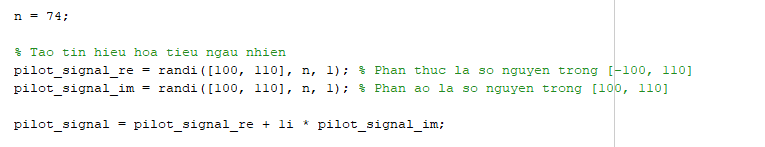
\includegraphics[width=14cm]{photo/5.1.1.png}
    \caption{Tạo tín hiệu hoa tiêu trong Matlab}
    \label{Hình 15}
\end{figure}\\
\begin{figure}[h!]
    \centering
    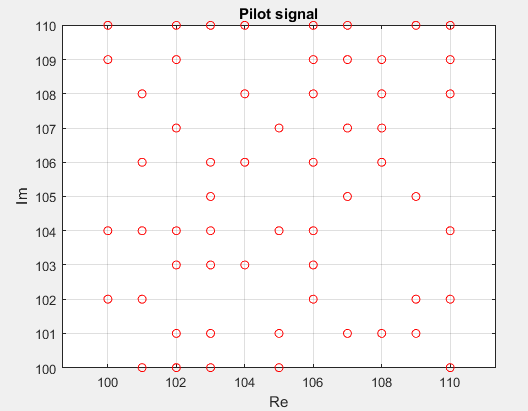
\includegraphics[width=14cm]{photo/5.1.2.png}
    \caption{Biểu diễn tín hiệu hoa tiêu trên mặt phẳng phức}
    \label{Hình 16}
\end{figure}

\subsection{Đọc tín hiệu quan sát}
Ở đây giả sử rằng bên thu sử dụng các thiết bị thu và đo đạc để tìm được các tín hiệu thu được và thống kê ở dạng file xlsx (file excel). Phần thực của tín hiệu quan sát được lưu trong đường dẫn \texttt{C:\textbackslash CE project\textbackslash yr.xlxs} . Phần ảo của tín hiệu quan sát được lưu trong đường dẫn \texttt{C:\textbackslash CE project\textbackslash yi.xlxs}. Để đọc dữ liệu và đổi kiểu dữ liệu về định dạng phù hợp và cộng phần ảo và phần thực lại với nhau ta dùng các lệnh sau:
\begin{figure}[h!]
    \centering
    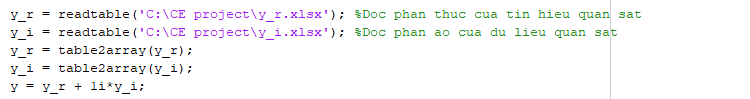
\includegraphics[width=14cm]{photo/5.2.1.png}
    \caption{Đọc và xử lý dữ liệu phía thu}
    \label{Hình 17}
\end{figure}\\
\begin{figure}[h!]
    \centering
   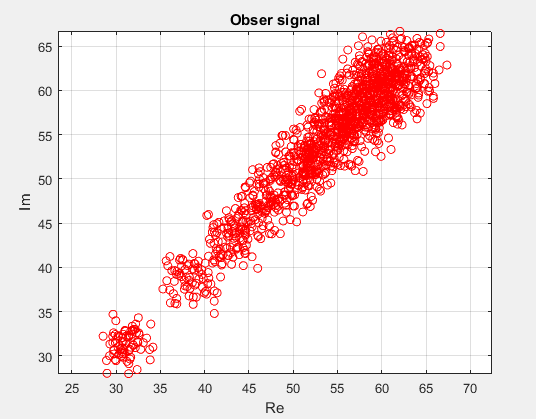
\includegraphics[width=12cm]{photo/5.2.2.png}
    \caption{Phân bố tín hiệu thu trên mặt phẳng phức}
    \label{Hình 18}
\end{figure}

\subsection{Ước lượng kênh truyền}
Do tín hiệu trong mô phỏng này là tín hiệu phức nên ta dùng công thức:
 $$\hat{h} = \frac{\overline{X}^H \overline{Y}}{\| \overline{X} ^2 \|} \text{ với } \begin{cases}
    x = (\text{pilot\_singal})^H  &\\
    \text{tu\_so} = \overline{X}^H.\overline{Y} &\\
    \text{mau\_so} = \|\overline{X}\|^2&
\end{cases}$$
\begin{figure}[h!]
    \centering
    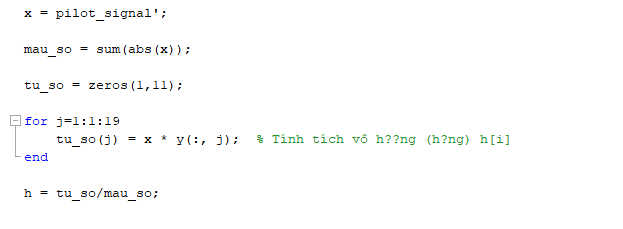
\includegraphics[width=14cm, height =6cm]{photo/5.3.1.png}
    \caption{Code tìm ước lượng kênh truyền}
    \label{Hình 19}
\end{figure}\\
\begin{figure}[h!]
    \centering
    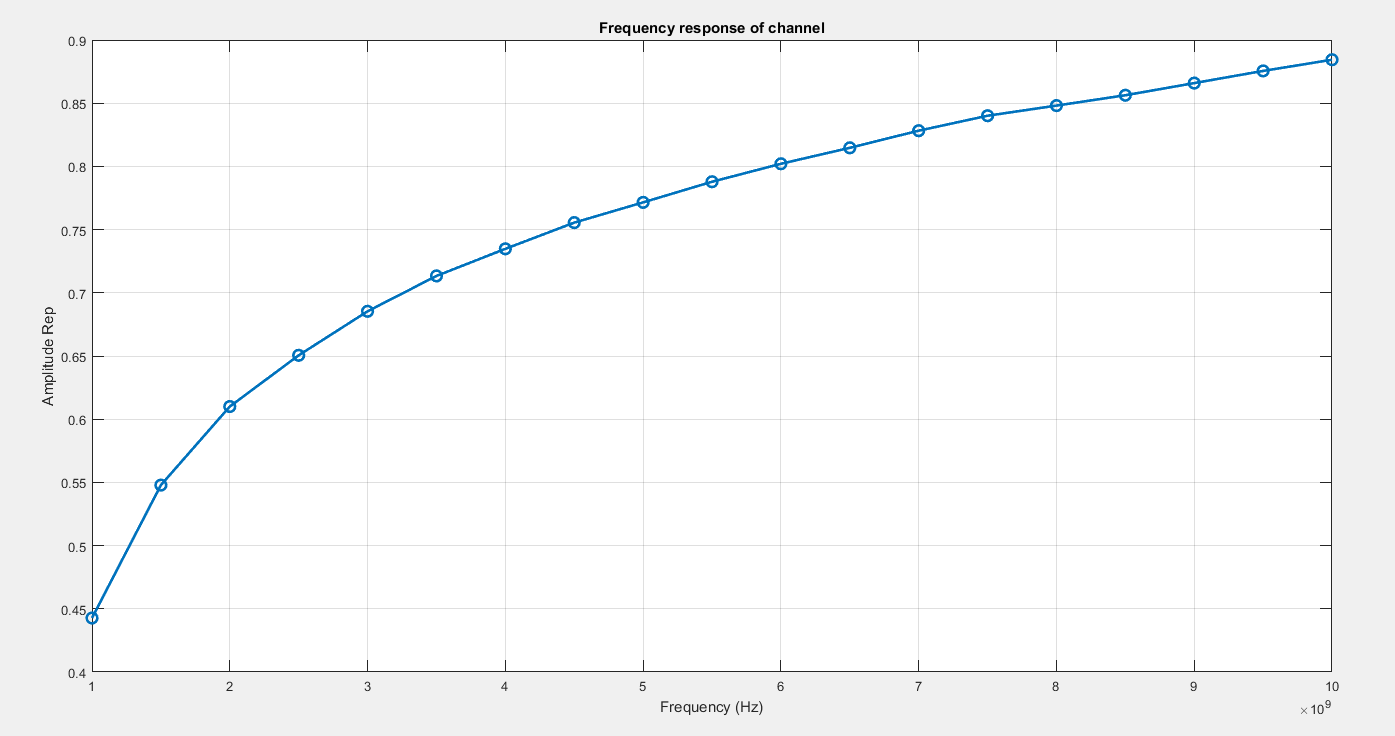
\includegraphics[width=13cm, height =11cm]{photo/5.3.2.png}
    \caption{Đáp ứng tần số của kênh truyền}
    \label{Hình 20}
\end{figure}
\newpage
Nhận xét: ta có thể thấy đáp ứng tần số của kênh truyền giả sử này là một đường cong "mượt". Do các tín hiệu hoa tiêu được giả sử khá lớn nên kênh truyền ít bị ảnh hưởng bởi nhiễu. Để thấy được sự ảnh hưởng của nhiễu lên kênh truyền khi tín hiệu hoa tiêu có công suất nhỏ ta cũng làm tương tự với các bước mô phỏng bên trên nhưng sẽ giảm độ lớn hay công suất của tín hiệu hoa tiêu.
\begin{figure}[h!]
    \centering
    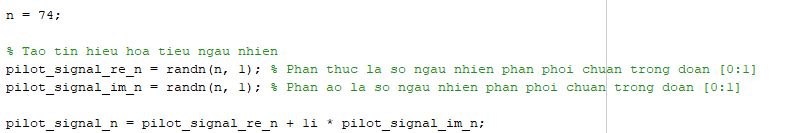
\includegraphics[width=14cm]{photo/5.3.3.png}
    \caption{Tạo tín hiệu hoa tiêu công suất nhỏ}
    \label{Hình 21}
\end{figure}\\
\begin{figure}[h!]
    \centering
    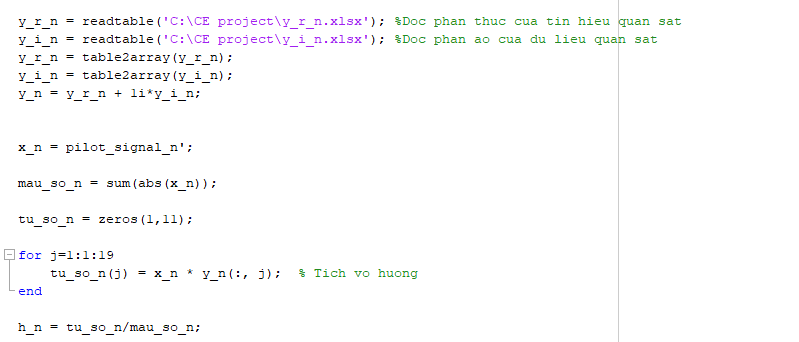
\includegraphics[width=14cm, height =7cm]{photo/5.3.4.png}
    \caption{Đọc tín hiệu quan sát khi bị ảnh hưởng nhiễu}
    \label{Hình 22}
\end{figure}\\
\begin{figure}[h!]
    \centering
    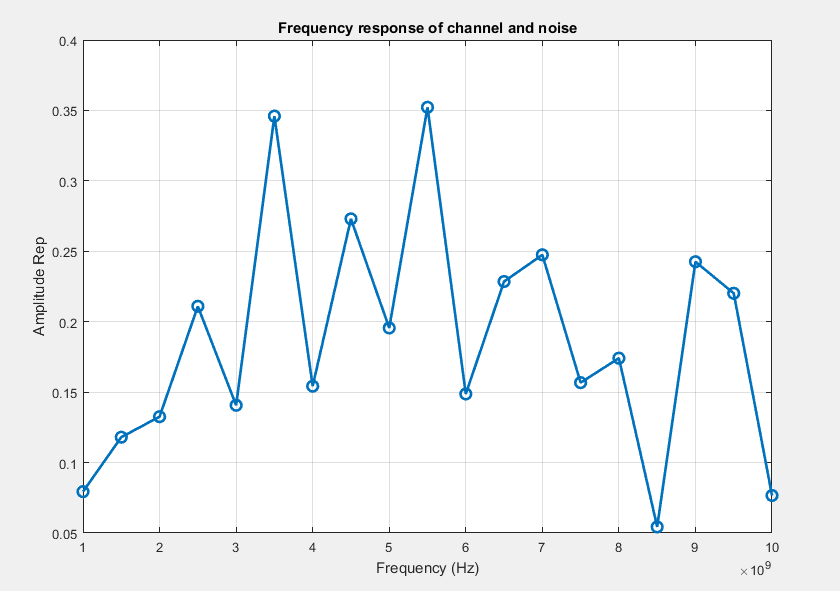
\includegraphics[width=14cm, height =6cm]{photo/5.3.5.png}
    \caption{Ước lượng kênh truyền bị ảnh hưởng nhiễu}
    \label{Hình 23}
\end{figure}

\section{Mô hình kênh truyền đa ngõ vào - một ngõ ra (Multiple Input Single Output - MISO}

Để phát triển thành mô hình đa ngõ vào, đa ngõ ra trước tiên ra cần xét mô hình đơn giản hơn là mô hình đa ngõ vào, một ngõ ra. Với mô hình đa ngõ vào, một ngõ ra bên nhận sẽ nhận nhiều tín hiệu từ nhiều nguồn khác nhau. Mỗi một nguồn phát tín hiệu khi đi đến bên nhận sẽ có một kênh truyền khác nhau từ $h_1, h_2,...h_m$. Mô hình này gặp rất nhiều trong thực tế. Giả sử như đài truyền hình, chúng ta chỉ cần một thiết bị thu sóng ví dụ như tivi, radio,.. để có thể nhận thông tin từ nhiều kênh truyền bằng cách điều chỉnh tần số nhận. Mỗi đâì truyền hình phát sóng với một khoảng băng thông khác nhau nên kênh truyền ảnh hưởng lên các sóng đó cũng là khác nhau. Vì vậy, chúng ta phải xây dựng mô hình ước lượng đồng thời các kênh truyền. 

\begin{figure}[h!]
    \centering
  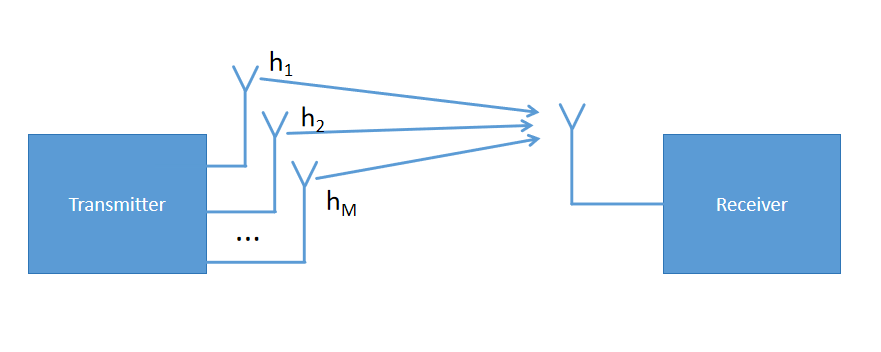
\includegraphics[width=14cm, height =6cm]{photo/6.1.png}
    \caption{Mô hình kênh truyền đa ngõ vào - một ngõ ra}
    \label{Hình 24}
\end{figure}
Với $M$ bên truyền, bên nhận sẽ có $M$ giá trị khác nhau do mỗi kênh truyền cần một tín hiệu hoa tiêu, vì vậy, chúng ta cần truyền một vector hoa tiêu kí hiệu là $x_i(k)$ là tín hiệu hoa tiêu của bên truyền $i$ tại thời điểm $k$. Vì vậy, giá trị quan sát $y(k)$ tại thời điểm $k$ sẽ là tổng các tín hiệu phát của kênh truyền tương ứng và nhiễu.
$$y(k) = h_1.x_1(k) + h_2.x_2(k)...+ h_M.x_M(k) + v(k)$$
$$y(k) = \begin{pmatrix}
    x_1(k)&x_2(k)&...&x_M(k)
\end{pmatrix} \begin{pmatrix}
    h_1\\h_2\\...\\h_M
\end{pmatrix} + v(k)$$

Xét tín hiệu quan sát tại nhiều thời điểm $y(1), y(2),..y(N)$ sẽ được mô hình theo ma trận truyền nhận, với số cột là một thời điểm được đo, mỗi hàng là một bên phát như sau:
$$\begin{pmatrix}
    y(1)\\y(2)\\y(3)\\...\\y(N)
\end{pmatrix} = \begin{pmatrix}
    x_1(1)&x_1(2)&x_1(3)&...&x_1(N)\\
    x_2(1)&x_2(2)&x_2(3)&...&x_2(N)\\
    x_3(1)&x_3(2)&x_3(3)&...&x_3(N)\\
    ...\\
    x_M(1)&x_M(2)&x_M(3)&...&x_1(N)\\
\end{pmatrix} \begin{pmatrix}
    h_1\\h_2\\h_3\\...\\h_M
\end{pmatrix} + \begin{pmatrix}
    v(1)\\v(2)\\v(3)\\...\\v(N)
\end{pmatrix}$$
$$ \overline{Y} = X\overline{h} + \overline{V}$$

Có thể thấy, trong mô hình đa ngõ vào, một ngõ ra thì giá trị của kênh truyền $\hat{h}$ được biểu diển ở dạng vector. Nên mô hình toán học của ước lượng lúc này sẽ không còn là ước lượng tham số mà sẽ trở thành ước lượng vector.

\section{Mô hình kênh truyền đa ngõ vào - đa ngõ ra (Multiple Input Multiple Output - MIMO}
Mô hình đa ngõ vào, đa ngõ ra là một hệ thống phức tạp vì các kênh truyển ảnh hưởng chéo lên nhau rất nhiều tạo ra can nhiễu lớn. Vì trong các trường hợp tổng quát, ta sẽ có rất nhiều bên phát và rất nhiều bên thu. Để dễ hình dung về kênh truyền MIMO, chúng ta xét bài toán hai ngõ vào, hai ngõ ra để dễ hình dung. Để mô hình kênh truyền về dạng toán học, ta gọi kênh truyền có dạng $h_{ij}$ với bên nhận thứ $i$ và bên phát thứ $j$

\begin{figure}[h!]
    \centering
    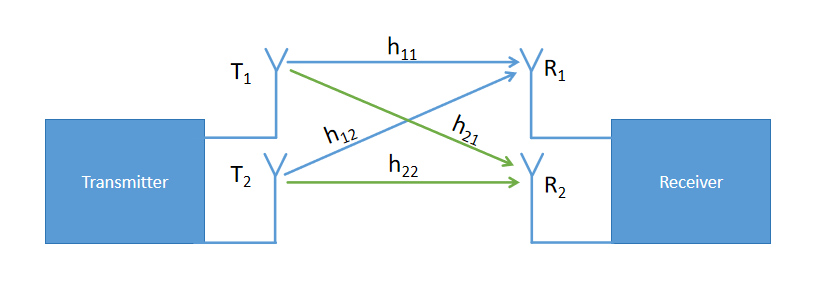
\includegraphics[width=14cm, height =6cm]{photo/7.1.png}
    \caption{Mô hình kênh truyền đa ngõ vào, đa ngõ ra}
    \label{Hình 25}
\end{figure}
Gọi $x_j$ là tín hiệu từ bên phát thứ $j$, $y_i$ là tín hiệu quan sát được từ bên nhận thứ $i$, $k$ là thời điểm phát hoặc thu được. Khi đó giá trị quan sát sẽ có dạng:
$$y_i(k) = h_{i1}.x_1(k) + h_{i2}.x_2(k) + h_{i3}.x_3(k) + ... + v_i(k)$$
Đơn giản hóa với mô hình hai ngõ vào, hai ngõ ra. Ta có giá trị quan sát như sau:
$$y_1(k) = h_{11}.x_1(k) + h_{12}.x_2(k) + v_1(k) $$
$$ y_2(k) = h_{21}.x_1(k) + h_{22}.x_2(k) + v_2(k)$$
Viết lại dưới dạng ma trận:
$$ \begin{pmatrix}
    y_1(k)\\y_2(k)
\end{pmatrix} = \begin{pmatrix}
    h_{11}&h_{12}\\
    h_{21}&h_{22}
\end{pmatrix} \begin{pmatrix}
    x_1(k)\\x_2(k)
\end{pmatrix} + \begin{pmatrix}
    v_1(k)\\v_2(k)
\end{pmatrix}$$
$$ \overline{y}(k) = H.\overline{x}(k) + \overline{V}(k)$$

Có thể thấy, trong mô hình đa ngõ vào, đa ngõ ra thì giá trị của kênh truyền $H$ được biểu diển ở dạng mở rộng hơn nữa là dạng ma trận. Nên mô hình toán học của ước lượng lúc này cũng sẽ không còn là ước lượng tham số hay vector mà sẽ trở thành ước lượng ma trận hay vector hai chiều. Giả sử bên phát sẽ phát $N$ vector hoa tiêu $\overline{x}(1),\overline{x}(2),...\overline{x}(N)$, ta có:
$$\overline{y}(1) = H.\overline{x}(1) + \overline{V}(1) $$
$$\overline{y}(2) = H.\overline{x}(2) + \overline{V}(2)$$
$$...$$
$$\overline{y}(N) = H.\overline{x}(N) + \overline{V}(N) \rightarrow Y = H.X +V$$

Bằng phương pháp bình phương cực tiểu và các mô hình toán học liên quan, ta tìm được ước lượng $\hat{H}$ có dạng ma trận, trong đó từng hàng và cột của ma trận kênh truyền sẽ là tương ứng với sự ảnh hưởng khác nhau của bên phát và bên thu.
$$\fcolorbox{red}{white}{$\hat{H} = Y.X^T.(X.X^T)^{-1}$}$$
\section{Mô phỏng kênh truyền MIMO trong MATLAB}
\subsection{Tạo tín hiệu hoa tiêu và tín hiệu quan sát}
Giả sử ta có hai nguồn phát và hai nguồn thu tín hiệu. Mỗi nguồn phát sử dụng 74 tín hiệu hoa tiêu có giá trị trong khoảng [95:100] và ta cũng dùng các công thức toán để tạo ra dữ liệu quan sát. Tại mỗi thời điểm $k$ ta giả sử phát một tần số nhất định, bắt đầu từ 1Mhz kết thúc là 2Mhz với bước nhảy là 500Khz. Ta thu được giá trị ước lượng của $H$ là một mảng 3 chiều

\begin{figure}[h!]
    \centering
      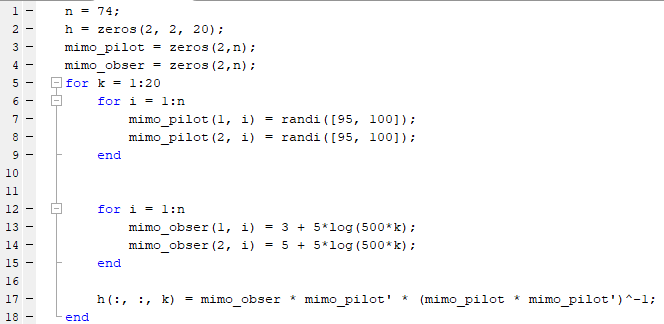
\includegraphics[width=14cm, height =6cm]{photo/8.1.1.png}\\
    \caption{Tạo tín hiệu hoa tiêu và tín hiệu quan sát cho mô hình MIMO}
    \label{Hình 26}
\end{figure}\\
\begin{figure}[h!]
    \centering
    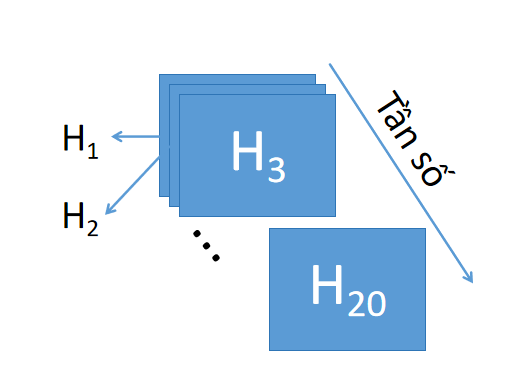
\includegraphics[width=9cm, height =7cm]{photo/8.1.2.png}
    \caption{Các ước lượng $H$ theo tần số}
    \label{Hình 27}
\end{figure}


\subsection{Ước lượng các kênh truyền}
Sau khi đã có các giá trị ước lượng kênh truyền $H$. Ta tiến hành vẽ đồ thị. Đồ thị của $H$ sẽ được vẽ bằng cách nối các $H_{ij}$ tương ứng với các $k$ khác nhau. Kết quả thu được của ước lượng kênh truyền hai ngõ vào, hai ngõ ra là 4 kênh truyền $H_{11},H_{12},H_{21},H_{22} $
\newpage
\begin{figure}[h!]
    \centering
    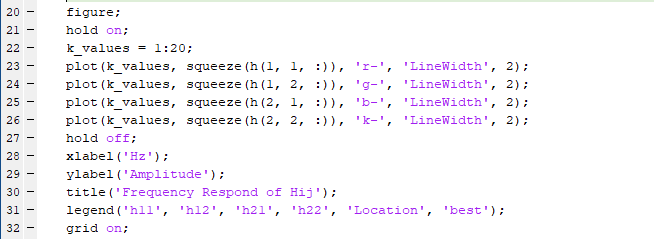
\includegraphics[width=14cm, height =7cm]{photo/8.2.1.png}
    \caption{Tạo đồ thị ước lượng $H$}
    \label{Hình 28}
\end{figure}\\
\begin{figure}[h!]
    \centering
    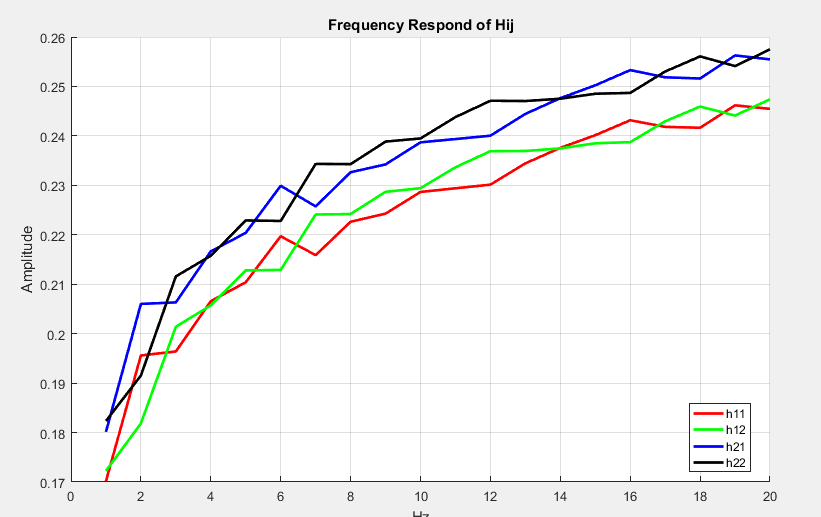
\includegraphics[width=14cm, height =9cm]{photo/8.2.2.png}
    \caption{Ước lượng kênh truyền MIMO}
    \label{Hình 29}
\end{figure}\\

Như đã nói trong thực tế, bên nhận có thể điều chỉnh bộ thu để nhận được tín hiệu từ nhiều kênh truyền khác nhau, vì vậy, ước lượng kênh truyền của tất cả các kênh phát là cần thiết trong thực tế. Mỗi kênh truyền có một giá trị khác nhau nên khi có các giá trị kênh truyền, phía thu có thể sử dụng các bộ cân bằng và khôi phục thích hợp với từng kênh truyền. 
\newpage
\section{Kết luận}
Nhìn chung, trong hệ thống viễn thông hiện đại, các kỹ thuật ước lượng kênh truyền là rất quan trọng và cần thiết trong việc nâng cao hiệu suất và khả năng điều khiển trong các hệ thống truyền thông. Với những tiến bộ không ngừng trong lĩnh vực lý thuyết và công nghệ, các phương pháp ước lượng này sẽ tiếp tục được cải tiến và mở rộng ứng dụng, đóng góp quan trọng vào sự phát triển của các hệ thống thông tin hiện đại\\

Trong đề tài này, chúng ta đã khám phá một loạt các kỹ thuật ước lượng kênh truyền trong các hệ thống truyền thông hiện đại. Mỗi phương pháp đều có những ưu điểm và nhược điểm riêng, và có thể được áp dụng tùy thuộc vào yêu cầu cụ thể của từng hệ thống.\\

Đầu tiên, chúng ta đã giới thiệu về các kỹ thuật ước lượng kênh truyền cơ bản như Ước lượng hợp lý cực đại và Compressed Sensing, cùng với những ứng dụng cụ thể của chúng trong thực tế. Trong khi Ước lượng hợp lý cực đại mang lại kết quả chính xác trong nhiều tình huống, thì Compressed Sensing lại là một lựa chọn hữu ích khi dữ liệu bị giới hạn hoặc yêu cầu tiết kiệm băng thông. Sau đó, bài viết cũng đi vào các phương pháp phức tạp hơn như Bộ lọc Kalman và Phương pháp dò tia. Các phương pháp khắc phục nhược điểm của ML và CS như không thích hợp trong kênh truyền NLoS hoặc môi trường động.\\

Tiếp theo, Chúng ta tìm hiểu sâu hơn vào phương pháp ML, áp dụng các lý thuyết ước lượng vào mô hình kênh truyền SISO, và mô phỏng các kênh truyền này trong MATLAB. Các kết quả mô phỏng cho thấy hiệu quả của phương pháp ước lượng ML trong việc tìm được đáp ứng biên độ của kênh truyền.\\

Cuối cùng, với việc mở rộng mô hình sang kênh truyền MIMO, chúng ta thực hiện mô phỏng kênh truyền MIMO trong MATLAB đã cung cấp những minh chứng rõ ràng cho việc có thể áp dụng các kỹ thuật ước lượng đã được trình bày. Với kiến thức còn hạn chế, nhóm đã cố gắng hoàn thành việc ước lượng kênh truyền MIMO như mục tiêu nhóm đặt ra từ lý thuyết cho đến mô phỏng.\\





\newpage
\section{Phụ lục code}
\lstset{
    basicstyle=\ttfamily\small, % Font code
    numbers=left,               % Đánh số dòng bên trái
    numberstyle=\tiny,          % Kích thước số dòng
    frame=single,               % Khung bao quanh code
    keywordstyle=\color{blue},  % Màu từ khóa
    commentstyle=\color{gray},  % Màu chú thích
    stringstyle=\color{red},    % Màu chuỗi
    breaklines=true,            % Tự động xuống dòng
}
\begin{lstlisting}[language=Matlab, caption=Kênh truyền ngõ vào đơn ngõ ra đơn]

n = 74;

% Tao tin hieu hoa tieu ngau nhien
pilot_signal_re = randi([100, 110], n, 1); % Phan thuc la so nguyen trong [-100, 110]
pilot_signal_im = randi([100, 110], n, 1); % Phan ao la so nguyen trong [100, 110]

pilot_signal = pilot_signal_re + 1i * pilot_signal_im;

% ma so
y_r = zeros(74,10);
y_i = zeros(74,10);

k = 1;
for j=10000000:500000:19000000 
    noise_re = randn(n,1);
    noise_im = randn(n,1);
    y_r(:,k) = (log(20*k)/10)*pilot_signal_re + noise_re;
    y_i(:,k) = (log(20*k)/10)*pilot_signal_im + noise_im;
    k = k+1;
   
end

y_r = readtable('C:\CE project\y_r.xlsx'); %Doc phan thuc cua tin hieu quan sat
y_i = readtable('C:\CE project\y_i.xlsx'); %Doc phan ao cua du lieu quan sat
y_r = table2array(y_r);
y_i = table2array(y_i);
y = y_r + 1i*y_i;

x = pilot_signal';

mau_so = sum(abs(x));

tu_so = zeros(1,11);

for j=1:1:19
    tu_so(j) = x * y(:, j);  
end

h = tu_so/mau_so;

h_a = abs(h/100);
x = 1:length(h_a);

figure; % T?o m?t c?a s? m?i cho ?? th?
plot(real(pilot_signal), imag(pilot_signal), 'ro'); 
title('Pilot signal');
xlabel('Re');
ylabel('Im');
grid on; 
axis equal;

figure; 
plot(real(y), imag(y), 'ro'); 
title('Obser signal');
xlabel('Re');
ylabel('Im');
grid on; 
axis equal;

f_start = 1e9; % 1 GHz
f_step = 0.5e9; % 50 kHz
frequencies = f_start + (x-1) * f_step; 

figure; 
plot(frequencies, h_a, '-o', 'MarkerSize', 8, 'LineWidth', 2); 
xlabel('Frequency (Hz)');
ylabel('Amplitude Rep'); 
title('Frequency response of channel'); 
grid on; 

n = 74;

% Tao tin hieu hoa tieu ngau nhien
pilot_signal_re_n = randn(n, 1); % Phan thuc la so ngau nhien phan phoi chuan trong doan [0:1]
pilot_signal_im_n = randn(n, 1); % Phan ao la so ngau nhien phan phoi chuan trong doan [0:1]

pilot_signal_n = pilot_signal_re_n + 1i * pilot_signal_im_n;


y_r_n = zeros(74,10);
y_i_n = zeros(74,10);

k = 1;
for j=10000000:500000:19000000 
    noise_re = randn(n,1);
    noise_im = randn(n,1);
    y_r_n(:,k) = (log(2*k)/10)*pilot_signal_re_n + noise_re;
    y_i_n(:,k) = (log(2*k)/10)*pilot_signal_im_n + noise_im;
    k = k+1;
   
end

y_r_n = readtable('C:\CE project\y_r_n.xlsx'); %Doc phan thuc cua tin hieu quan sat
y_i_n = readtable('C:\CE project\y_i_n.xlsx'); %Doc phan ao cua du lieu quan sat
y_r_n = table2array(y_r_n);
y_i_n = table2array(y_i_n);
y_n = y_r_n + 1i*y_i_n;

x_n = pilot_signal_n';

mau_so_n = sum(abs(x_n));

tu_so_n = zeros(1,11);

for j=1:1:19
    tu_so_n(j) = x_n * y_n(:, j);  % Tich vo huong
end

h_n = tu_so_n/mau_so_n;

h_a_n = abs(h_n);
x = 1:length(h_a_n);

f_start = 1e9; % 1 GHz
f_step = 0.5e9; % 50 kHz
frequencies = f_start + (x-1) * f_step; % Tinh vector tan so

figure; 
plot(frequencies, h_a_n, '-o', 'MarkerSize', 8, 'LineWidth', 2); 
xlabel('Frequency (Hz)'); 
ylabel('Amplitude Rep'); 
title('Frequency response of channel and noise'); 
grid on; 

\end{lstlisting}


\begin{lstlisting}[language=Matlab, caption=Kênh truyền đa ngõ vào đa ngõ ra]
n = 74;
h = zeros(2, 2, 20);
mimo_pilot = zeros(2,n);
mimo_obser = zeros(2,n);
for k = 1:20
    for i = 1:n
        mimo_pilot(1, i) = randi([99, 100]);  
        mimo_pilot(2, i) = randi([99, 100]);  
    end

    for i = 1:n
        mimo_obser(1, i) = 3 + 5*log(500*k);  
        mimo_obser(2, i) = 5 + 5*log(500*k); 
    end

    h(:, :, k) = mimo_obser*mimo_pilot'*(mimo_pilot*mimo_pilot')^-1;
end

figure; 
hold on; 
k_values = 1:20; 
plot(k_values, squeeze(h(1, 1, :)), 'r-', 'LineWidth', 2); 
plot(k_values, squeeze(h(1, 2, :)), 'g-', 'LineWidth', 2); 
plot(k_values, squeeze(h(2, 1, :)), 'b-', 'LineWidth', 2); 
plot(k_values, squeeze(h(2, 2, :)), 'k-', 'LineWidth', 2); 
hold off; 
xlabel('Hz');
ylabel('Amplitude');
title('Frequency Respond of Hij');
legend('h11', 'h12', 'h21', 'h22', 'Location', 'best');
grid on; 

\end{lstlisting}

\section{Tài liệu kham khảo}
\href{ https://commsbrief.com/difference-between-mimo-siso-simo-and-miso-antenna-systems/ }{1. Adnan Ghayas, \textit{"Difference Between MIMO, SISO, SIMO, and MISO Antenna Systems"}, Commsbrief, October 30, 2021} \\

\href{ https://www.researchgate.net/publication/297833789_Sparse_Channel_Estimation_Based_on_Compressed_Sensing_for_Massive_MIMO_Systems }{2. Chenhao Qi,Yongming Huang
Shi Jin and Lenan Wu,\textit{"Sparse Channel Estimation Based on Compressed Sensing for Massive MIMO Systems"}, IEEE International Conference on Communications (ICC 2015), IEEE Communications Letters, June 2015} \\

\href{ https://www.researchgate.net/publication/337969126_Deep_Learning_Based_Channel_Estimation_Algorithm_for_Fast_Time-Varying_MIMO-OFDM_Systems }{3. Yong Liao and Yuanxiao Hua, \textit{"Deep Learning Based Channel Estimation Algorithm for Fast Time-Varying MIMO-OFDM Systems"},IEEE Communications Letters, December 2019} \\

\href{ https://www.nature.com/articles/s41467-024-47865-6 }{4. Jing Cheng Liang, Lei Zhang, Zhangjie Luo, Rui Zhe Jiang, Zhang Wen Cheng, Si Ran Wang, Meng Ke Sun, Shi Jin, Qiang Cheng and Tie Jun Cui, \textit{"A filtering reconfigurable intelligent surface for interference-free wireless communications"}, Nature Communications, 07 May 2024} \\

\href{ https://info.support.huawei.com/info-finder/encyclopedia/en/MIMO.html }{5. Wang Yibo, \textit{"What Is MIMO?"}, Huawei Info Finder Encyclopedia, 2024-05-31} \\

\href{ https://www.hs-osnabrueck.de/fileadmin/HSOS/Forschung/Recherche/Laboreinrichtungen_und_Versuchsbetriebe/Labor_fuer_Hochfrequenztechnik_und_Mobilkommunikation/Forschung/digitale_Funksysteme/Channel-Estimation.pdf }{6. HS Osnabrück, \textit{"Channel estimation"}, Osnabrück University of Applied Sciences} \\

\href{ https://www.youtube.com/watch?v=ZsLh01nlRzY&t=3s }{7. Iain Explains, \textit{"Basics of Channel Estimation for Mobile Communications"}, Macquarie University in Sydney, 08/11/2021} \\

\href{ https://ieeexplore.ieee.org/document/8640815 }{8. Mehran Soltani, Vahid Pourahmadi, Ali Mirzaei and Hamid Sheikhzadeh, \textit{"Deep Learning for Channel Estimation in MIMO Systems"}, IEEE Communications Letters, 12 February 2019} \\

\href{ https://kth.diva-portal.org/smash/get/diva2:538857/FULLTEXT01.pdf }{9. Idd Pazi Alli, \textit{"Channel Estimation in Mobile Wireless Systems"}, KTH Sweden} \\

\href{ https://machinelearningcoban.com/2017/07/17/mlemap/ }{10.  Machine Learning cơ bản, \textit{"Maximum Likelihood và Maximum A Posteriori estimation"}, Jul 17, 2017} \\

\href{ https://www.mathworks.com/help/lte/ug/channel-estimation.html }{\textit{"Channel estimation"}, MathWorks} \\

\href{ https://www.mathworks.com/help/signal/ug/signal-generation-and-visualization.html }{\textit{11. "Signal Generation and Visualization"}, MathWorks} \\

\href{ https://www.mathworks.com/help/comm/ref/txsite.raytrace.html }{12. \textit{"Raytrace, Display or compute RF propagation rays"}, MathWorks} \\

\href{ http://tailieuso.udn.vn/bitstream/TTHL_125/8428/2/NguyenThiDieuHan.TT.pdf }{13. Nguyen Thi Dieu Han, \textit{"Ước Lượng Kênh Truyền cho Truyền Dẫn OFDM Sử Dụng Phương Pháp Maximum Likelihood"}, Da Nang University of Science and Technology, 21/06/2015} \\

\href{ https://www.academia.edu/51012261/Analysis_and_Optimization_of_Fast_Channel_Estimation_In_Millimeter_Wave_Vehicular_Communication }{14. Aani RS, Akshai RK, Anakha Venugopal, C Krishna and Hema \textit{"Different Types of Channel Estimation Techniques Used in MIMO-OFDM for Effective Communication Systems"}, IOSR Journal of Engineering, 8, August 2021} \\

\href{ https://www.youtube.com/playlist?list=PL1qOdYF_cLbqSpbZfp51Xo-J-5REr1UCg }{15. Satyaki Roy, \textit{"Estimation for Wireless Communications MIMO And Sensor Networks"}, Indian Institute of Technology Kanpur} \\

\href{ https://viblo.asia/p/so-luoc-ve-maximum-likelihood-estimation-1Je5EvrYKnL }{16. Tran Duc Tan, \textit{"Sơ lược về Maximum Likelihood Estimation"}, VIBLO, 22/07/2019} \\

\href{ https://www.mdpi.com/2075-5309/4/2/113 }{17. Sönke Pelzer, Lukas Aspöck, Dirk Schröder and Michael Vorländer, \textit{"Integrating Real-Time Room Acoustics Simulation into a CAD Modeling Software to Enhance the Architectural Design Process"}, Licensee MDPI, Basel, Switzerland, 21 April 2014} \\

\href{ https://www.mdpi.com/1424-8220/22/16/5971 }{18. Mohammad Abrar Shakil Sejan, Md Habibur Rahman and Md Habibur Rahman, \textit{"Demod-CNN: A Robust Deep Learning Approach for Intelligent Reflecting Surface-Assisted Multiuser MIMO Communication"},Licensee MDPI, Basel, Switzerland, 10 August 2022} \\

\href{ https://en.wikipedia.org/wiki/Channel_state_information }{\textit{19. "Channel state information"}, Wikipedia} \\


\end{document}
